\chapter{Propagating Sentinel-2 Top-of-Atmosphere Radiometric Uncertainty into Land Surface Phenology Metrics Using a Monte Carlo Framework}
\label{chap:uncertainty}
\graphicspath{{./04-Uncertainty/img}}

Lukas Valentin Graf\textsuperscript{1,2}, Javier Gorro\~{n}o\textsuperscript{3}, Andreas Hueni\textsuperscript{4}, Achim Walter\textsuperscript{1}, Helge Aasen\textsuperscript{1,2}
\\
\normalsize
\vspace{2pt}
\\
\textit{\textsuperscript{1}Group of Crop Science, Institute of Agricultural Sciences, Department of Environmental Systems Science, ETH Zurich, Universitätstrasse 2 , 8092 Zurich, Switzerland
\\
\textsuperscript{2}Earth Observation of Agroecosystems Team, Devision Agroecology and Environment,\ Agroscope, Reckenholzstrasse 191, CH-8042 Zürich, Switzerland
\\
\textsuperscript{3}Research Institute of Water and Environmental Engineering (IIAMA), Universitat Politècnica de València, Camino de Vera, s/n ES-46022 Valencia, Spain
\\
\textsuperscript{4}Remote Sensing Laboratories, Department of Geography, University of Zurich, Winterthurerstrasse 190. CH-8057 Zürich, Switzerland
\vspace{0.1cm}}
\\

The following chapter contains a pre-print of the paper with the same title published in \textsl{IEEE Journal of Selected Topics in Applied Earth Observations and Remote Sensing} with the doi: \doi{10.1109/JSTARS.2023.3297713} under the Creative Commons Attribution License CC BY 4.0 (\url{http://creativecommons.org/licenses/by/4.0/}).

% the file
\section*{Abstract}
Time series of optical imagery allow to derive land surface phenology metrics. These metrics are only complete with a statement about their uncertainty. A source of uncertainty is the radiometry of the sensor. We propagated radiometric uncertainties within a Monte-Carlo framework into phenological metrics using the TIMESAT approach based on time series of the Normalized Difference Vegetation Index (\gls{NDVI} ), three-band Enhanced Vegetation Index (\gls{EVI} ) and Green Leaf Area Index (GLAI) derived from radiative transfer modelling. Additionally, we studied the effect of propagated uncertainties on scene pre-classification. We focused on Sentinel-2 \gls{MSI} \gls{TOA}data since quantitative estimates of radiometric uncertainties are available. Propagation was carried out for a growing season over an agricultural region in Switzerland. Propagated uncertainties had little impact on the classification except for spectrally mixed pixels. Effects on the spectral indices and \gls{GLAI} were more pronounced. In detail, \gls{GLAI} was more uncertain due to the ill-posedness of radiative transfer model inversion (median relative uncertainty for all crop pixels and Sentinel-2 scenes: 4.4\%) than \gls{EVI} (2.7\%) and \gls{NDVI} (1.1\%). Regarding phenology, metrics exhibited largest uncertainties in the case of GLAI. The magnitude of uncertainty in the metrics depends on the inter-scene error correlation, which we assumed to be either zero (uncorrelated) or one (fully correlated) since the actual correlation is unknown. If uncertainties are fully correlated, uncertainties in metrics are small (2 to 3 days) but take values up to greater 10 days under the uncorrelated assumption. Thus, our work provides guidance for the interpretation of phenological metrics.

\section{Introduction}
\label{sec:unc_introduction}
Satellite remote sensing is of paramount importance for studying global environmental changes. More than four decades of optical remote sensing have generated a wealth of image and time series data that have made a significant contribution to the understanding of vegetation dynamics \citep{gonsamo_circumpolar_2016,caparros-santiago_land_2021, wu_development_2021}. From local to global scales, remote sensing-based canopy greenness proxies \citep{myneni_interpretation_1995} and derived functional traits \citep{verhoef_remote_2003,homolova_review_2013} provide the ability to quantify the effects of environmental factors on plant physiology over time \citep{melaas_detecting_2013,bolton_continental-scale_2020,croft_global_2020,tian_calibrating_2021}. Seasonal patterns of remote sensing data of vegetation are mostly summarised under the term "\gls{LSP}" \citep{de_beurs_land_2004}. \gls{LSP} has been extended to a set of metrics linking observed temporal changes in the spectral properties of vegetation to distinctive physiological transition phases \citep{zeng_review_2020}. Examples of these are \gls{SOS} and \gls{EOS} \citep{lloyd_phenological_1990,reed_measuring_1994}, which mark the onset of the growing season after winter and its end, respectively. Both metrics have therefore been used intensively in agricultural \citep{sakamoto_crop_2005,meroni_phenology-based_2014,gao_toward_2017,diao_remote_2020,salinero-delgado_monitoring_2022}, forestry \citep{melaas_detecting_2013,white_remote_2014,kowalski_characterizing_2020,shen_regional_2021} and ecological studies \citep{wagenseil_assessing_2006,gu_characterizing_2009,vrieling_vegetation_2018,moon_multiscale_2021}. For agriculture, such metrics are of increasing importance since different crops have strongly differing phenologies. Partly, the phenology depends on intrinsic properties of the crop. For example, winter wheat often is sown in October in the northern hemisphere, whereas maize or other summer crops are sown in spring. Moreover, field management and environmental conditions (drought, hail etc.) affect the crops' development and the precise analysis of crop phenology is an important tool for insurance assessments or for decision support when it comes to management issues such as finding the right time for fertilization.

In the past, sensors like MOderate Resolution Imaging Spectroradiometer (MODIS) or Advanced Very High Resolution Radiometer (AVHRR) were mainly used for \gls{LSP} studies. These have a high temporal but only a low spatial resolution ($\ge250$ m), which leads to spectral mixing effects \citep{helman_land_2018} and lack of spatial detail. With the Copernicus \gls{S2} mission, in addition to enhanced spatial resolution (up to $10$ m), the twin constellation of Sentinel-2A and -2B has improved temporal resolution remarkably (up to three days at mid-latitudes), making \gls{S2} data a valuable data source for \gls{LSP} studies and agricultural applications \citep{bolton_continental-scale_2020,tian_calibrating_2021,moon_multiscale_2021,amin_prototyping_2021,pazur_national_2022}. The \gls{MSI} on board the \gls{S2} satellites has 13 spectral bands, ten of which are suitable for remote sensing of land surfaces. By placing three spectral bands in the red-edge, two bands in the near-infrared, and two short-wave infrared bands, the \gls{S2}-\gls{MSI} instrument is suitable for vegetation studies \citep{frampton_evaluating_2013, misra_status_2020} and the accurate derivation of plant ecophysiological traits such as the \gls{GLAI}. This extends vegetation mapping capabilities beyond wide-spread spectral indices of canopy greenness such as the \gls{NDVI} \citep{rouse_monitoring_1974} or the \gls{EVI} \citep{huete_overview_2002}. \gls{S2} data is, for instance, used operationally to derive the Copernicus Pan-European High Resolution Vegetation Phenology and Productivity layer\footnote{\url{https://land.copernicus.eu/en/products/vegetation}}.

Despite the clear importance and widespread use of remote sensing data, our understanding of uncertainty in remotely sensed products such as \gls{LSP} is still poor albeit \cite{white_real-time_2006} already stressed the lack of remote sensing uncertainty estimates more than one decade ago. Furthermore, the Quality Assurance Framework for Earth Observation (QA4EO) endorsed by Committee on Earth Observation Satellites (CEOS) which has recently been extended by a joint effort of ESA and NASA \citep{hunt_quality_2021} highlights the need for uncertainty assessment of \gls{EO}-derived products such as \gls{LSP}. Only with a quantification of the sources of uncertainty (uncertainty budget), traceable and complete data products can be generated that allow users to evaluate the products for their fitness for purpose and indicate the uncertainty of their own analyses. Here, we focus on a source of uncertainty in \gls{LSP} metrics derived from \gls{S2}-\gls{MSI} data which, to the best of our knowledge, has hardly been considered so far: Uncertainty in the \gls{TOA} at-sensor-radiance values ($L_{at\_sensor}$). Any remote sensing product necessarily builds on \gls{TOA} radiances. Uncertainties in the radiometry is translated all the way down to the \gls{LSP} metrics and define the limits of the achievable uncertainty. \cite{mittaz_applying_2019} concluded that no uncertainty propagation from raw data to higher level products has been conducted so far along an \gls{EO} data processing chain. Moreover, the authors called for advancing \gls{EO} practice using approaches from metrologia. A first step towards closing this gap is therefore taken with the present work on the propagation of radiometric uncertainty.

Radiometric uncertainty is influenced by a set of uncertainty sources that derive from different contributions including both the instrument and the ground processing chain. Some of these contributions include, for example, the instrument noise or the solar diffuser used for on-board calibration \citep{gorrono_radiometric_2017}. In turn, these contributions can affect pixel-based uncertainty with different levels of correlation in the spatial, temporal, and spectral domain \citep{gorrono_providing_2018}. Uncertainties of $0.1$ to $1.5$ K are known from remote sensing of sea surface temperature \citep{merchant_sea_2014}, for example, while relative radiometric uncertainties of up to $5\%$ have been found in remote sensing of ocean color due to random effects \citep{melin_uncertainty_2016,mckinna_approach_2019}. It is therefore reasonable to assume that uncertainties in the radiometry of \gls{S2}-\gls{MSI} which take about 1 to 2\% \citep{gorrono_providing_2018} also have an impact on derived data products such as \gls{LSP} metrics.

The objective of this work is to propagate radiometric uncertainty from \gls{S2}-\gls{MSI} \gls{TOA} (L1C) data into \gls{LSP} metrics (L3) using widely used image processing resources focusing on an intensively farmed agricultural study area in Switzerland for a single growing season (Section \ref{sec:studyarea_data}). Swiss agriculture operates with small field sizes (average farm size 2020: 21 ha) of a larger number of crops next to each other. This high diversity is difficult to manage and satellite-based solutions for management decision support are therefore urgently required.
Spatial, temporal and spectral uncertainty contributors are propagated using a \gls{MC} framework as recommended in Supplement 1 to the Guide to the Expression of Uncertainty in Measurement (GUM, \citep{bipm_supplement_2008}) and implemented, for example, by \cite{gorrono_radiometric_2017} and \cite{gorrono_providing_2018}. Starting with the L1C data, we propagate the radiometric uncertainty through the atmospheric correction into bottom-of-atmosphere (BOA, i.e., processing level L2A) reflectance factor values. From the BOA reflectance factors, we derive the two most widely used spectral vegetation indices: \gls{NDVI} and EVI. Furthermore, we estimate the ecophysiological development of plants using \gls{GLAI}, which we determine from inversion of a radiative transfer model. Based on the uncertainties in \gls{NDVI}, \gls{EVI}, and \gls{GLAI}, we construct vegetation time series and derive \gls{SOS} and \gls{EOS} and their uncertainty in days. In addition, we test the effect of propagated uncertainties on the \gls{SCL} output by the L2A processor. The complete method outline is presented in Section \ref{sec:unc_methods} followed by a presentation (Section \ref{sec:unc_results}) and discussion of the results obtained (Section \ref{sec:unc_discussion}).

% definition of terms
\section{Terms and Definitions}
\label{sec:terms-and-definitions}
To avoid ambiguity in terms we provide definitions here: We define the term "uncertainty" as the degree of doubt about the reported \gls{TOA} reflectance values which is referred to as the best estimate. "Error", in contrast, is the difference between the measured value and the true, unknown \gls{TOA}reflectance value and splits into random and systematic components. Systematic errors can be minimized by pre- and post-launch calibration activities \citep{wyatt_radiometric_1978} while random errors can be suppressed by a sufficiently large sample size. Residual, i.e., uncorrected random and systematic error contribute to the overall radiometric uncertainty budget. Following the specification of the GUM, uncertainty estimates represent a confidence interval for a given probability distribution function (PDF) whose mean corresponds to the measured \gls{TOA}reflectance value. Standard uncertainty is defined as the interval around the mean of the uncertainty PDF that provides a coverage of 68.27\% ($k=1$) of possible realizations. In equations we denote the standard uncertainty with the Greek letter $\mu$ to be consistent with the GUM. All findings in this work are reported as standard uncertainties. To obtain uncertainty values with a higher coverage factor $k$ (i.e., multiple standard deviations), the uncertainties must be multiplied by $k$, for example to obtain uncertainties for $k=2$ used in instrument certification.

\section{Study Area and Data}
\label{sec:studyarea_data}
\subsection{Study Area}
We selected an intensively farmed study area located around the agricultural research station at Eschikon ($8.69 E, 47.45 N$) operated by ETH Zurich , north-east of the city of Zurich, Switzerland (see Figure \ref{fig:figure1-overview-map}). The study area is bound by a square with an approximated area of 100 $km^2$ (Figure \ref{fig:figure1-overview-map}A). With an average annual precipitation of 1241 mm and an air temperature of 10.1 deg C (reference period 2004 to 2022, based on a weather station\footnote{\url{https://www.agrometeo.ch/}} located at Strickhof-Lindau placed in the north-western part of the study area), the study region is representative for cropping conditions in the Swiss Central Plain, but also for geographically adjacent areas in Central and Western Europe.

A crop-type map showing the main crop per field parcel for the year 2019 was available from the administration of the canton of Zurich. The parcel boundaries and their crop type are shown in Figure \ref{fig:figure1-overview-map}A. To avoid spectral mixing effects at the parcel boundaries all geometries were buffered 20 m inwards. Parcels too small for the buffering operation were dropped from the database. In total, 2021 field parcels with 9 different crop types and two types of grassland were available. Most parcels are small; the median parcel size was about 0.19 ha (0.44 ha on average). Table \ref{tab:crop-area} shows the approximate area per crop type in hectares with winter wheat (228.8 ha) occupying the largest area.

\begin{figure*}
    \centering
    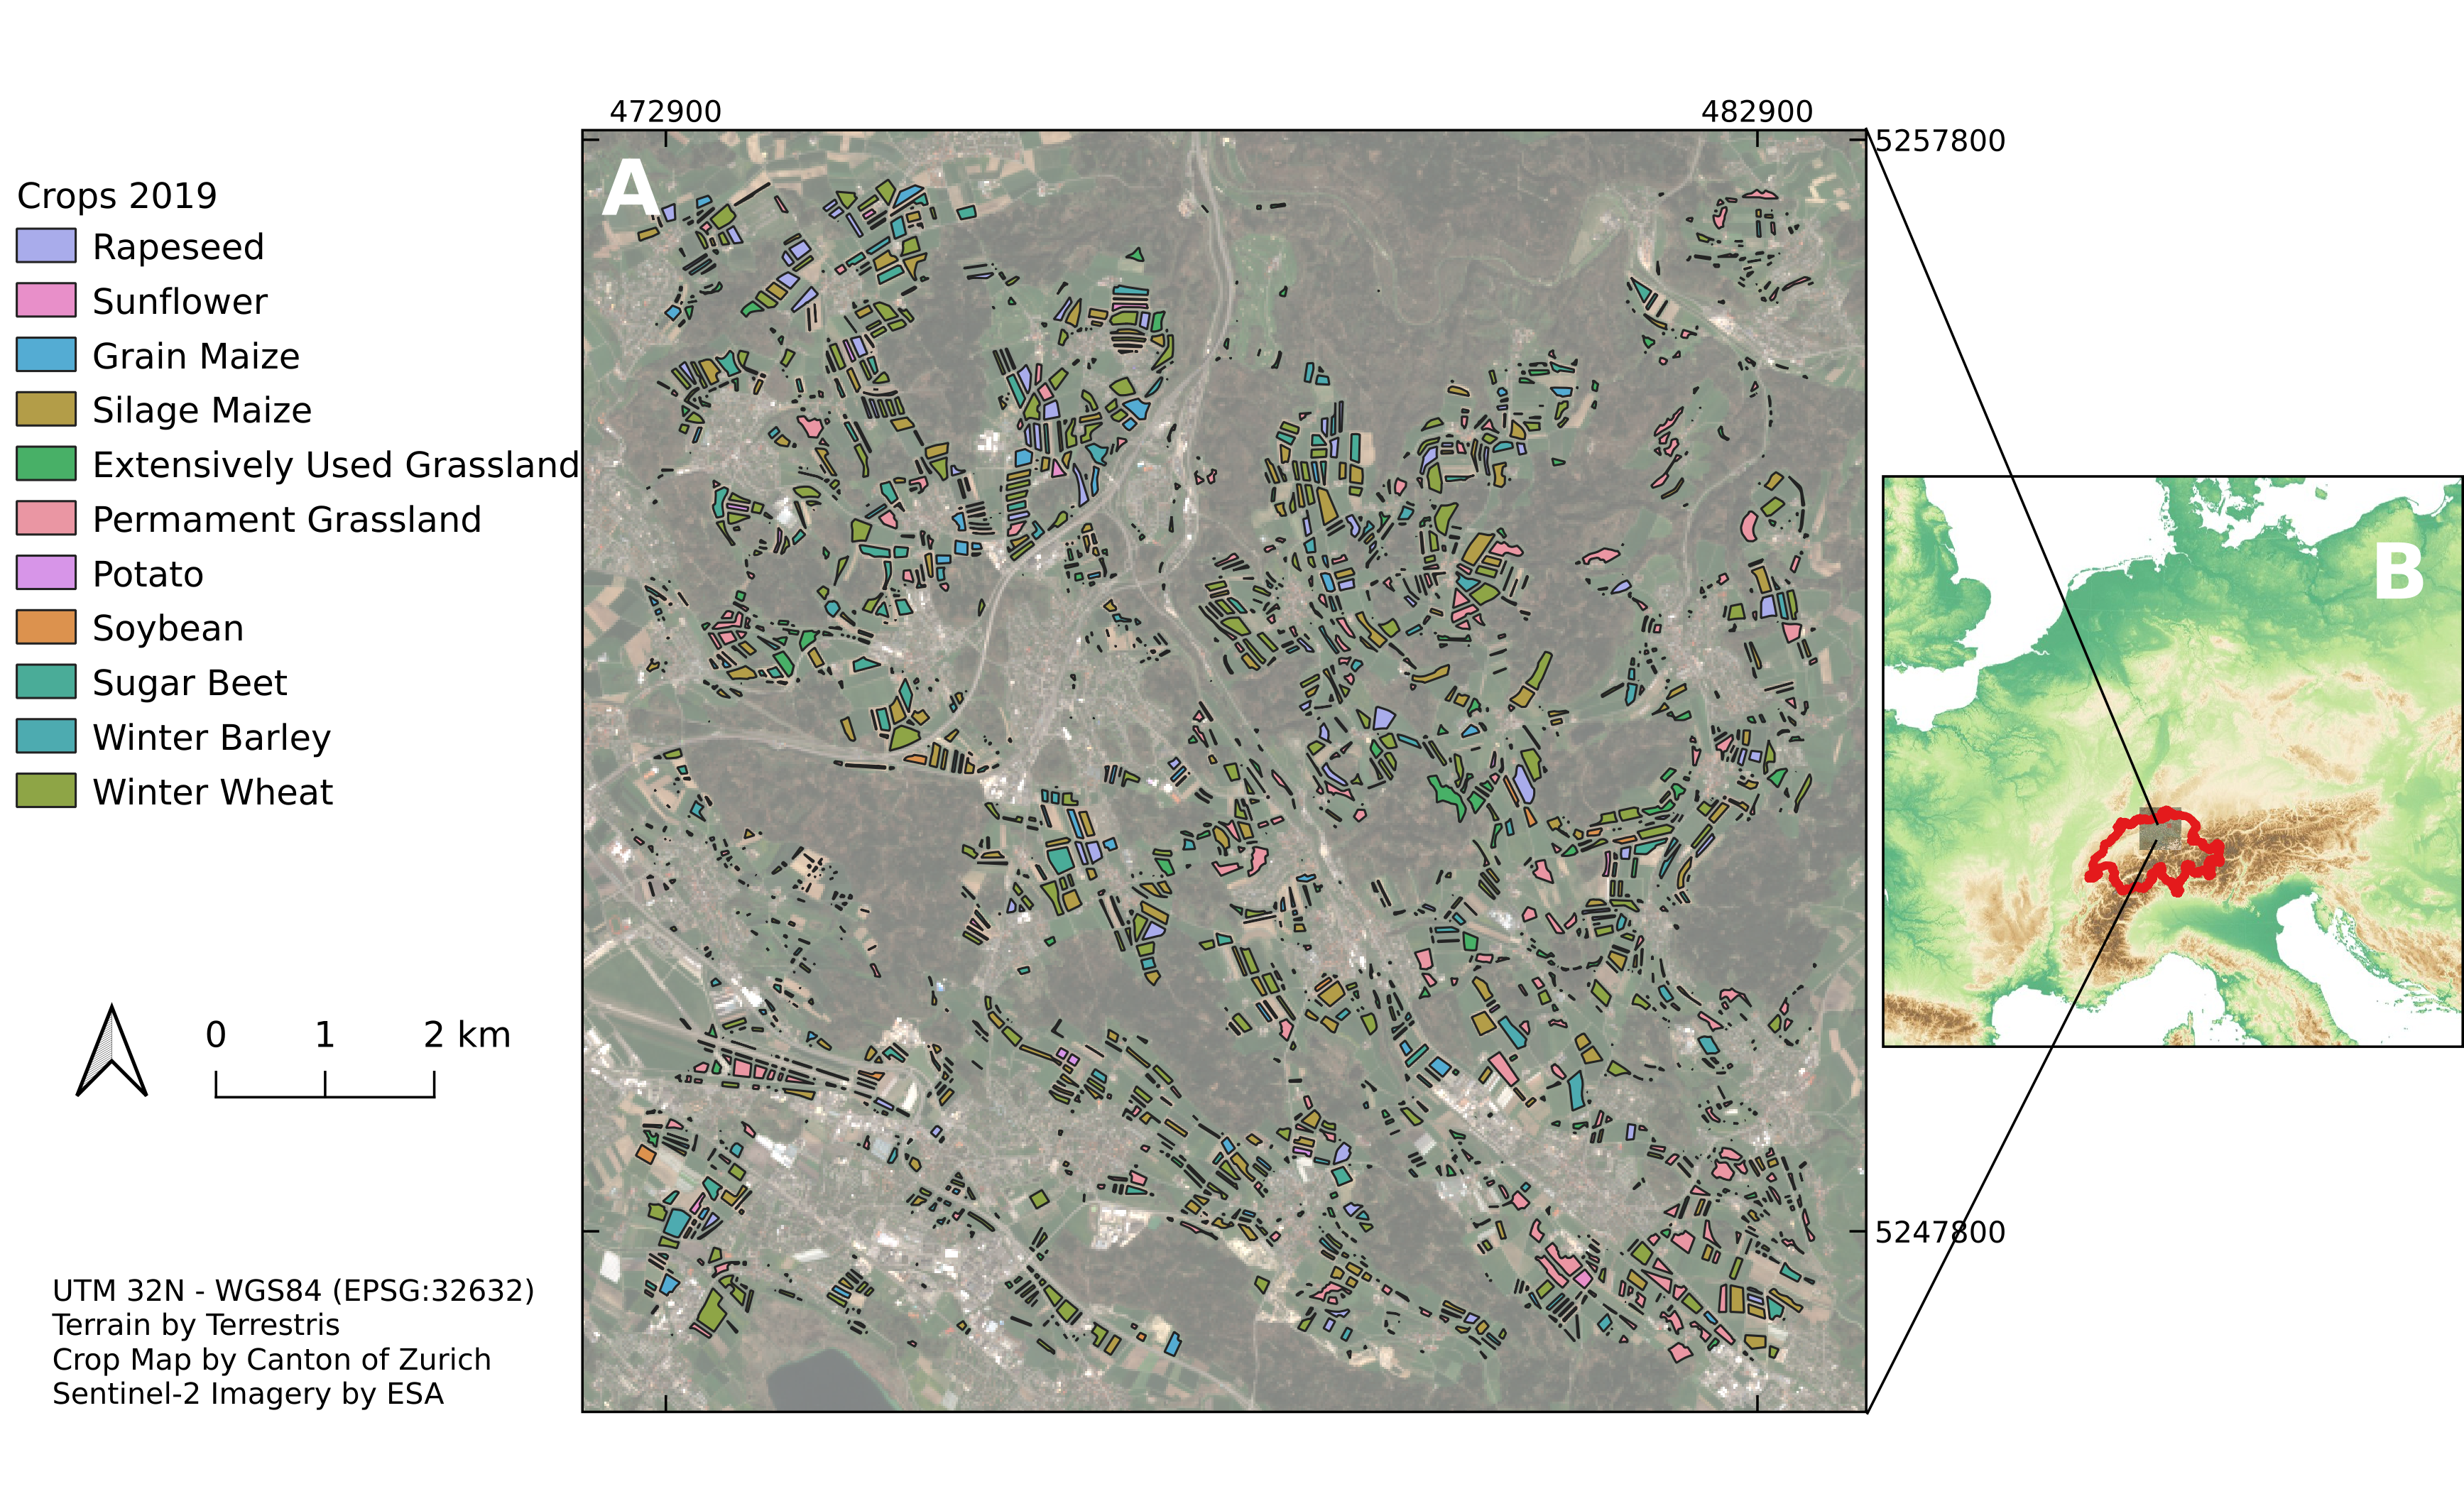
\includegraphics[width=1.0\textwidth]{Figure_1-Overview-Study-Area}
    \caption{Map of the study area with the field parcel geometries buffered 20 m inwards and their main crop types in 2019 (A) and the location of the Sentinel-2 tile T32TMT and the study region in Western Europe (B).}
    \label{fig:figure1-overview-map}
\end{figure*}

\begin{table}[!t]
    \centering
     \caption{Area per crop type in hectares in this study after buffering all field parcels 20 m inwards to avoid spectral mixing effects.}
    \begin{tabular}{lr}
    \toprule
    {} &   Area [ha] \\
    Crop Type                 &        \\
    \midrule
    Rapeseed                    &   70.4 \\
    Grain Maize                      &   41.3 \\
    Extensively Used Grasland &   62.9 \\
    Permament Grasland        &  168.9 \\
    Potato                    &    4.7 \\
    Silage Maize              &  175.6 \\
    Soybean                   &    7.8 \\
    Sugar Beet                &   65.4 \\
    Sunflower                 &    7.9 \\
    Winter Barley             &   63.4 \\
    Winter Wheat              &  228.8 \\
    \bottomrule
    \end{tabular}
    \label{tab:crop-area}
\end{table}

    
\subsection{Data}
We acquired 34 \gls{S2}-{MSI} \gls{TOA}scenes (L1C product) over the study area (\gls{S2} granule 32TMT, Figure \ref{fig:figure1-overview-map}B) from the Data and Information Access Service (DIAS) CREODIAS\footnote{\url{https://finder.creodias.eu/}} covering a time period from February 1st to October 15th 2019. All scenes had a scene-wide cloud coverage of $\le20\%$ which was used as a filtering criterion. This threshold is lower than reported in the literature for phenology retrieval. It was chosen to ensure that cloud and shadow contamination did not affect uncertainty propagation.
Figure \ref{fig:s2-scenes} shows the \gls{S2}scenes used and their cloudy pixel percentage derived from the metadata. The spacecraft (S2A or S2B) is denoted as blue and red dots, respectively. The PDGS (\gls{S2} Payload Data Ground Segment) processing baseline of the \gls{S2}scenes was 02.07 (N0207) for all scenes before July \nth{16} 2019, and 02.08 (N0208) after that date. According to the technical guide \footnote{\url{https://sentinels.copernicus.eu/web/sentinel/technical-guides/sentinel-2-msi/processing-baseline}} the change in baseline only affected the formatting of the instrument telemetry metadata. Therefore, we do not assume an impact of the baseline change on radiance values.

\begin{figure*}
    \centering
    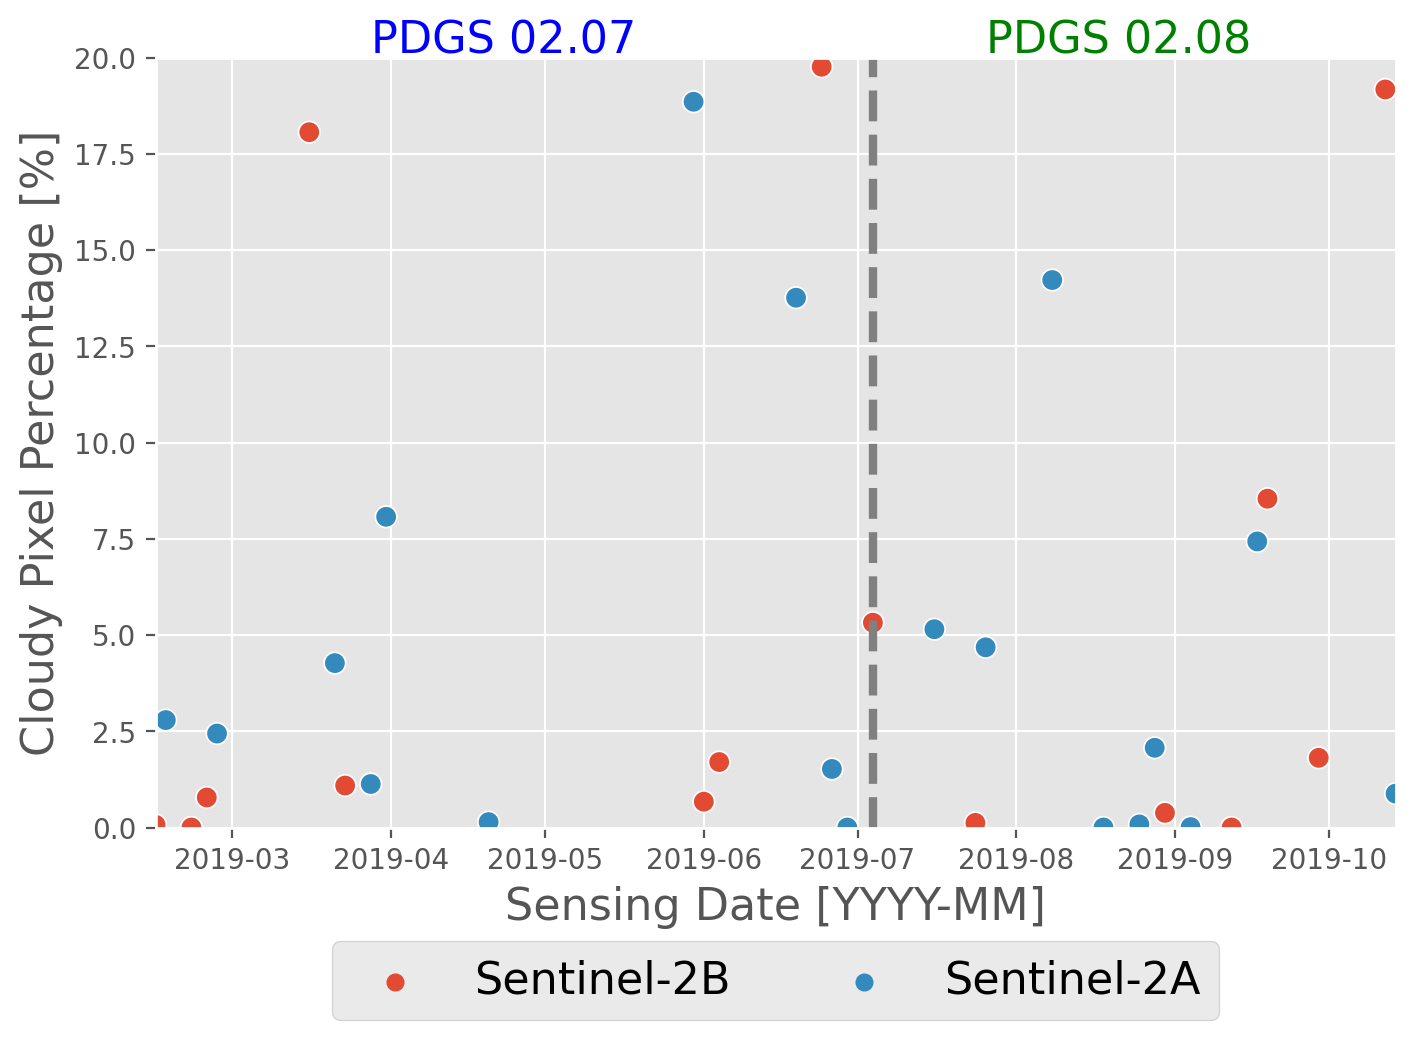
\includegraphics[width=1.0\textwidth]{Fig_S2-Data-Availability.png}
    \caption{S2 scenes used plotted against their scene-wide cloudy pixel percentage. Red dots denotes observations made by S2B, blue dots represent S2A scenes. The two different PDGS processing baselines are separated by the grey dashed line.}
    \label{fig:s2-scenes}
\end{figure*}


\section{Methods}
\label{sec:unc_methods}

In the following the manuscript is structured along the workflow in Figure \ref{fig:figure2-workflow}. Figure \ref{fig:figure2-workflow} shows the entire radiometric uncertainty propagation chain - starting from the L1C \gls{TOA}S2 scenes to uncertainties in the \gls{LSP} metrics (CEOS processing level L3). The individual steps from Figure \ref{fig:figure2-workflow} are explained in detail in the following sections (\ref{subsec:s2-rut} - \ref{subsec:time-series-scenarios}). Complementary to the uncertainty propagation workflow the total uncertainty budget of the \gls{LSP} metrics is shown in an uncertainty tree diagram in Figure \ref{fig:unc-diagram}. The diagram visualizes the context the radiometric uncertainty propagation chain is embedded into as explained in Section \ref{subsec:uncertainty-tree-diagram}.

\begin{figure*}
    \centering
    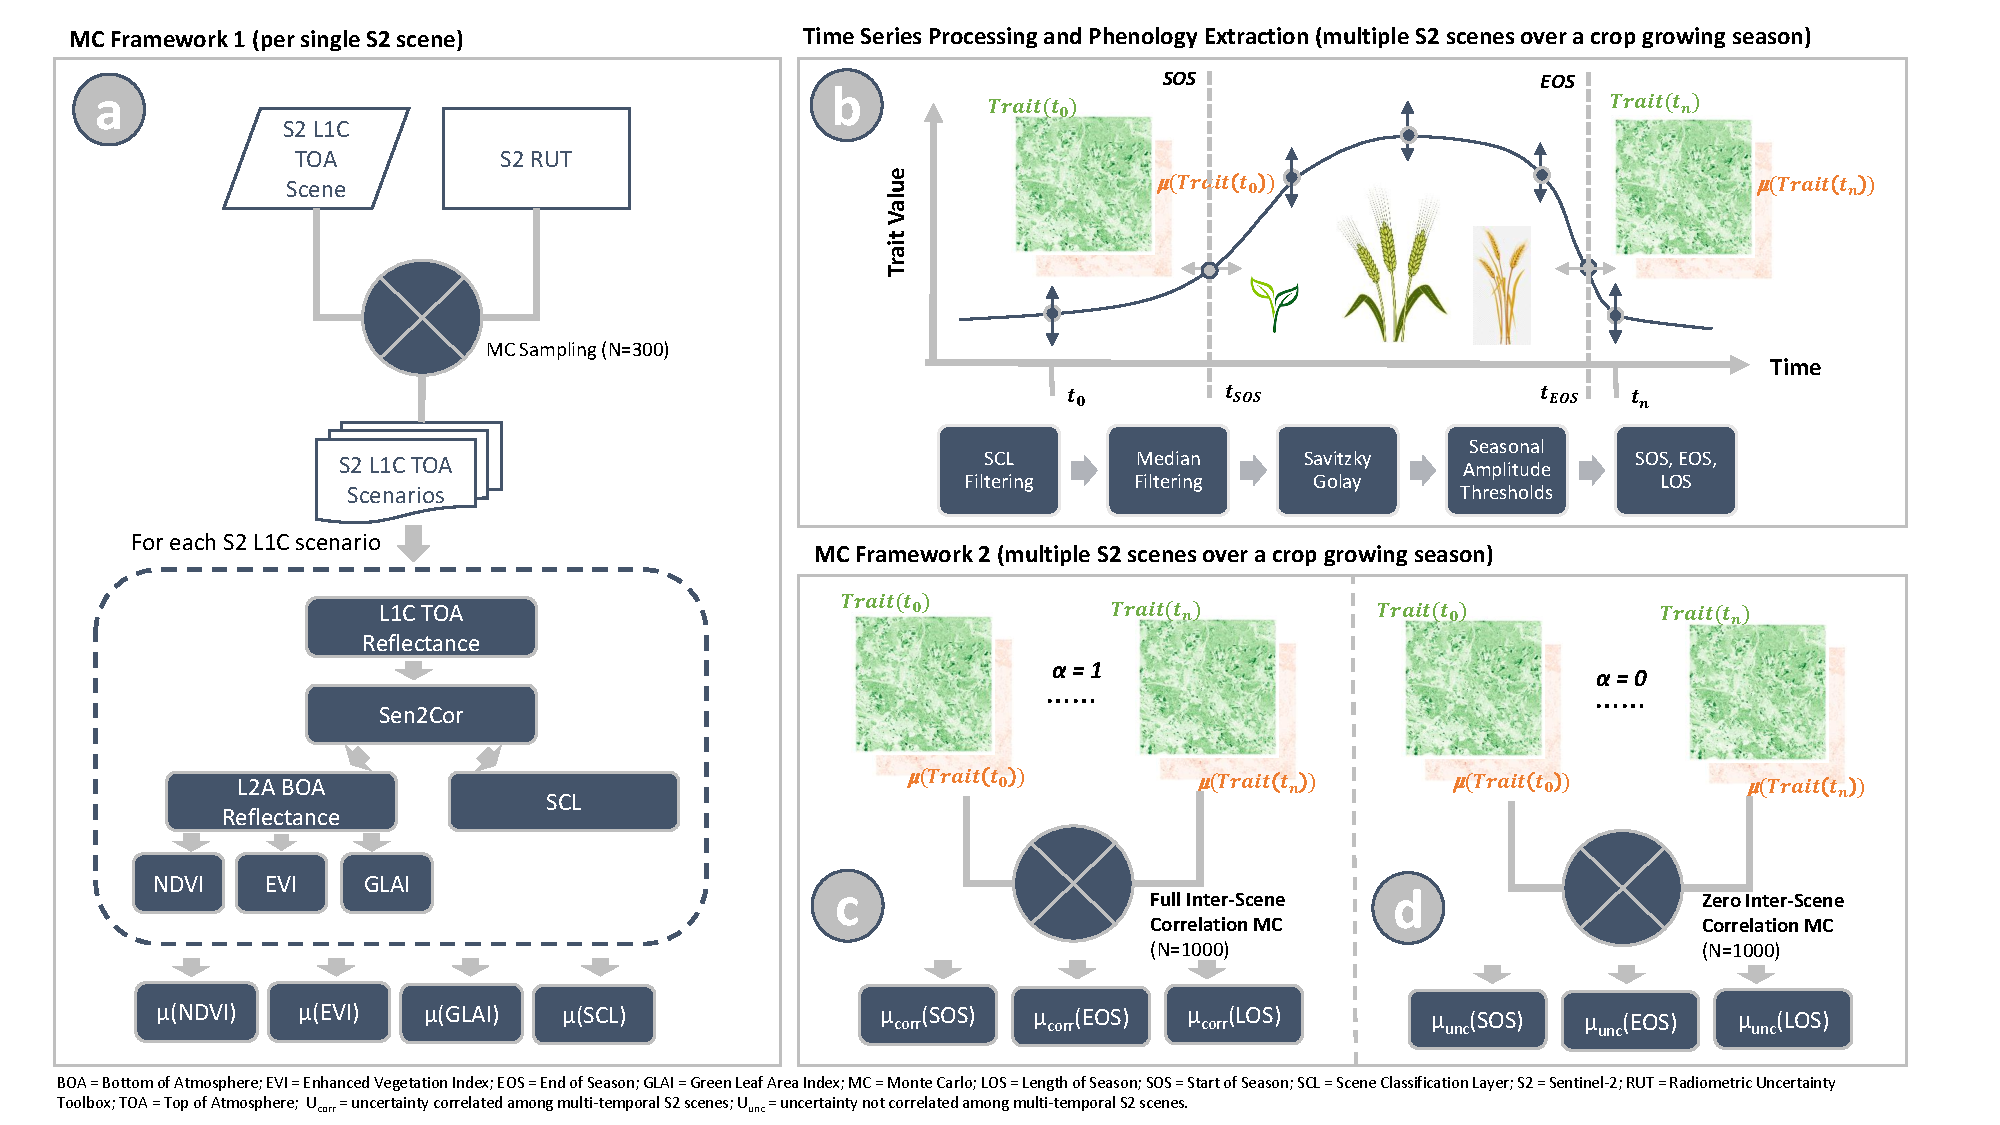
\includegraphics[width=\textwidth]{Figure_2-Workflow.pdf}
    \caption{Overview of the workflow for uncertainty ($\mu$) propagation. Using the \gls{S2-RUT} radiometric uncertainties are propagated from \gls{TOA}reflectance factors through atmospheric correction into NDVI, \gls{EVI} and \gls{GLAI} as well as \gls{SCL} uncertainty in a first \gls{MC} framework working on single \gls{S2}scenes (a). Multiple ($n$) \gls{S2}scenes acquired over an entire growing season are processed to obtain \gls{LSP} metrics from a trait (e.g., \gls{NDVI}) time series (b). Uncertainties obtained in the first  \gls{MC} framework are feed into (b) for a second  \gls{MC} sampling to derive \gls{LSP} uncertainty. Inter-scene (i.e., multi-temporal) error correlation is set to full correlation (c) and zero correlation (d) to include the two possible extreme cases for \gls{LSP} uncertainty retrieval.}
    \label{fig:figure2-workflow}
\end{figure*}

\subsection{Uncertainty Tree Diagram}
\label{subsec:uncertainty-tree-diagram}
Uncertainty tree diagrams represent the uncertainty budget of a measurement and trace back sources of uncertainty to their causing effects \citep{ma_uncertainty_2020,mittaz_applying_2019}. Uncertainty tree diagrams are complementary to workflow illustrations, such as the one in Figure \ref{fig:figure2-workflow} depicting the origin and entanglement of uncertainties. Figure \ref{fig:unc-diagram} shows an uncertainty tree diagram for the \gls{LSP} metrics. Starting from the final product (LSP metrics in the large blue box in Figure \ref{fig:unc-diagram}), sources of uncertainty are plotted along paths. Partial derivatives represent sensitivity coefficients. For example, $\frac{\partial LSP}{\partial NDVI}$ represents the sensitivity of uncertainty in the \gls{LSP} metrics to uncertainty in NDVI. Sources of uncertainty that cannot be quantified at this time are included in the total budget with $\mu(0)$, i.e., these contributions are set to zero, although their actual contribution is most likely $> 0$.

Uncertainty in the \gls{LSP} metrics depends not only on the parameterization of the time series model (light blue colored parts in Figure \ref{fig:unc-diagram}) but also on uncertainties in the spectral indexes (\gls{EVI}  or NDVI) or biophysical parameters (GLAI, pink colored parts in Figure \ref{fig:unc-diagram}) used. Here, it should be noted that EVI, \gls{NDVI} and \gls{GLAI} are alternative ways to derive the \gls{LSP} metrics. All these in turn depend on the uncertainty in the L2A product, which includes uncertainties in the L2A BOA reflectance factors, as well as the resulting uncertainties in the scene pre-classification (green colored parts in Figure \ref{fig:unc-diagram}). The uncertainty in the L2A product ultimately results from the uncertainty in the L1C \gls{TOA}reflectance factors (dark blue parts in Figure \ref{fig:unc-diagram}). Their uncertainty can be determined by means of the \gls{S2-RUT} (\cite{gorrono_radiometric_2017}, dashed border in Figure \ref{fig:unc-diagram}, upper left). The uncertainty sources shown in the \gls{S2-RUT} include effects whose uncertainties are thus propagated through the entire \gls{EO} processing pipeline.

Besides the radiometric uncertainty propagation path, there are other effects that contribute uncertainties to the uncertainty budget of the \gls{LSP} metrics. Examples are uncertainties in the \gls{GLAI} retrieval due to uncertainty in the RTM used or the uncertainty of the atmospheric correction in the L2A data. Therefore, all contributions except the radiometric uncertainty derived from the \gls{S2-RUT} are set to zero, since the quantification of the other uncertainties is far beyond the scope of this paper (see also Section \ref{subsec:limitations}).

\begin{figure*}
    \centering
    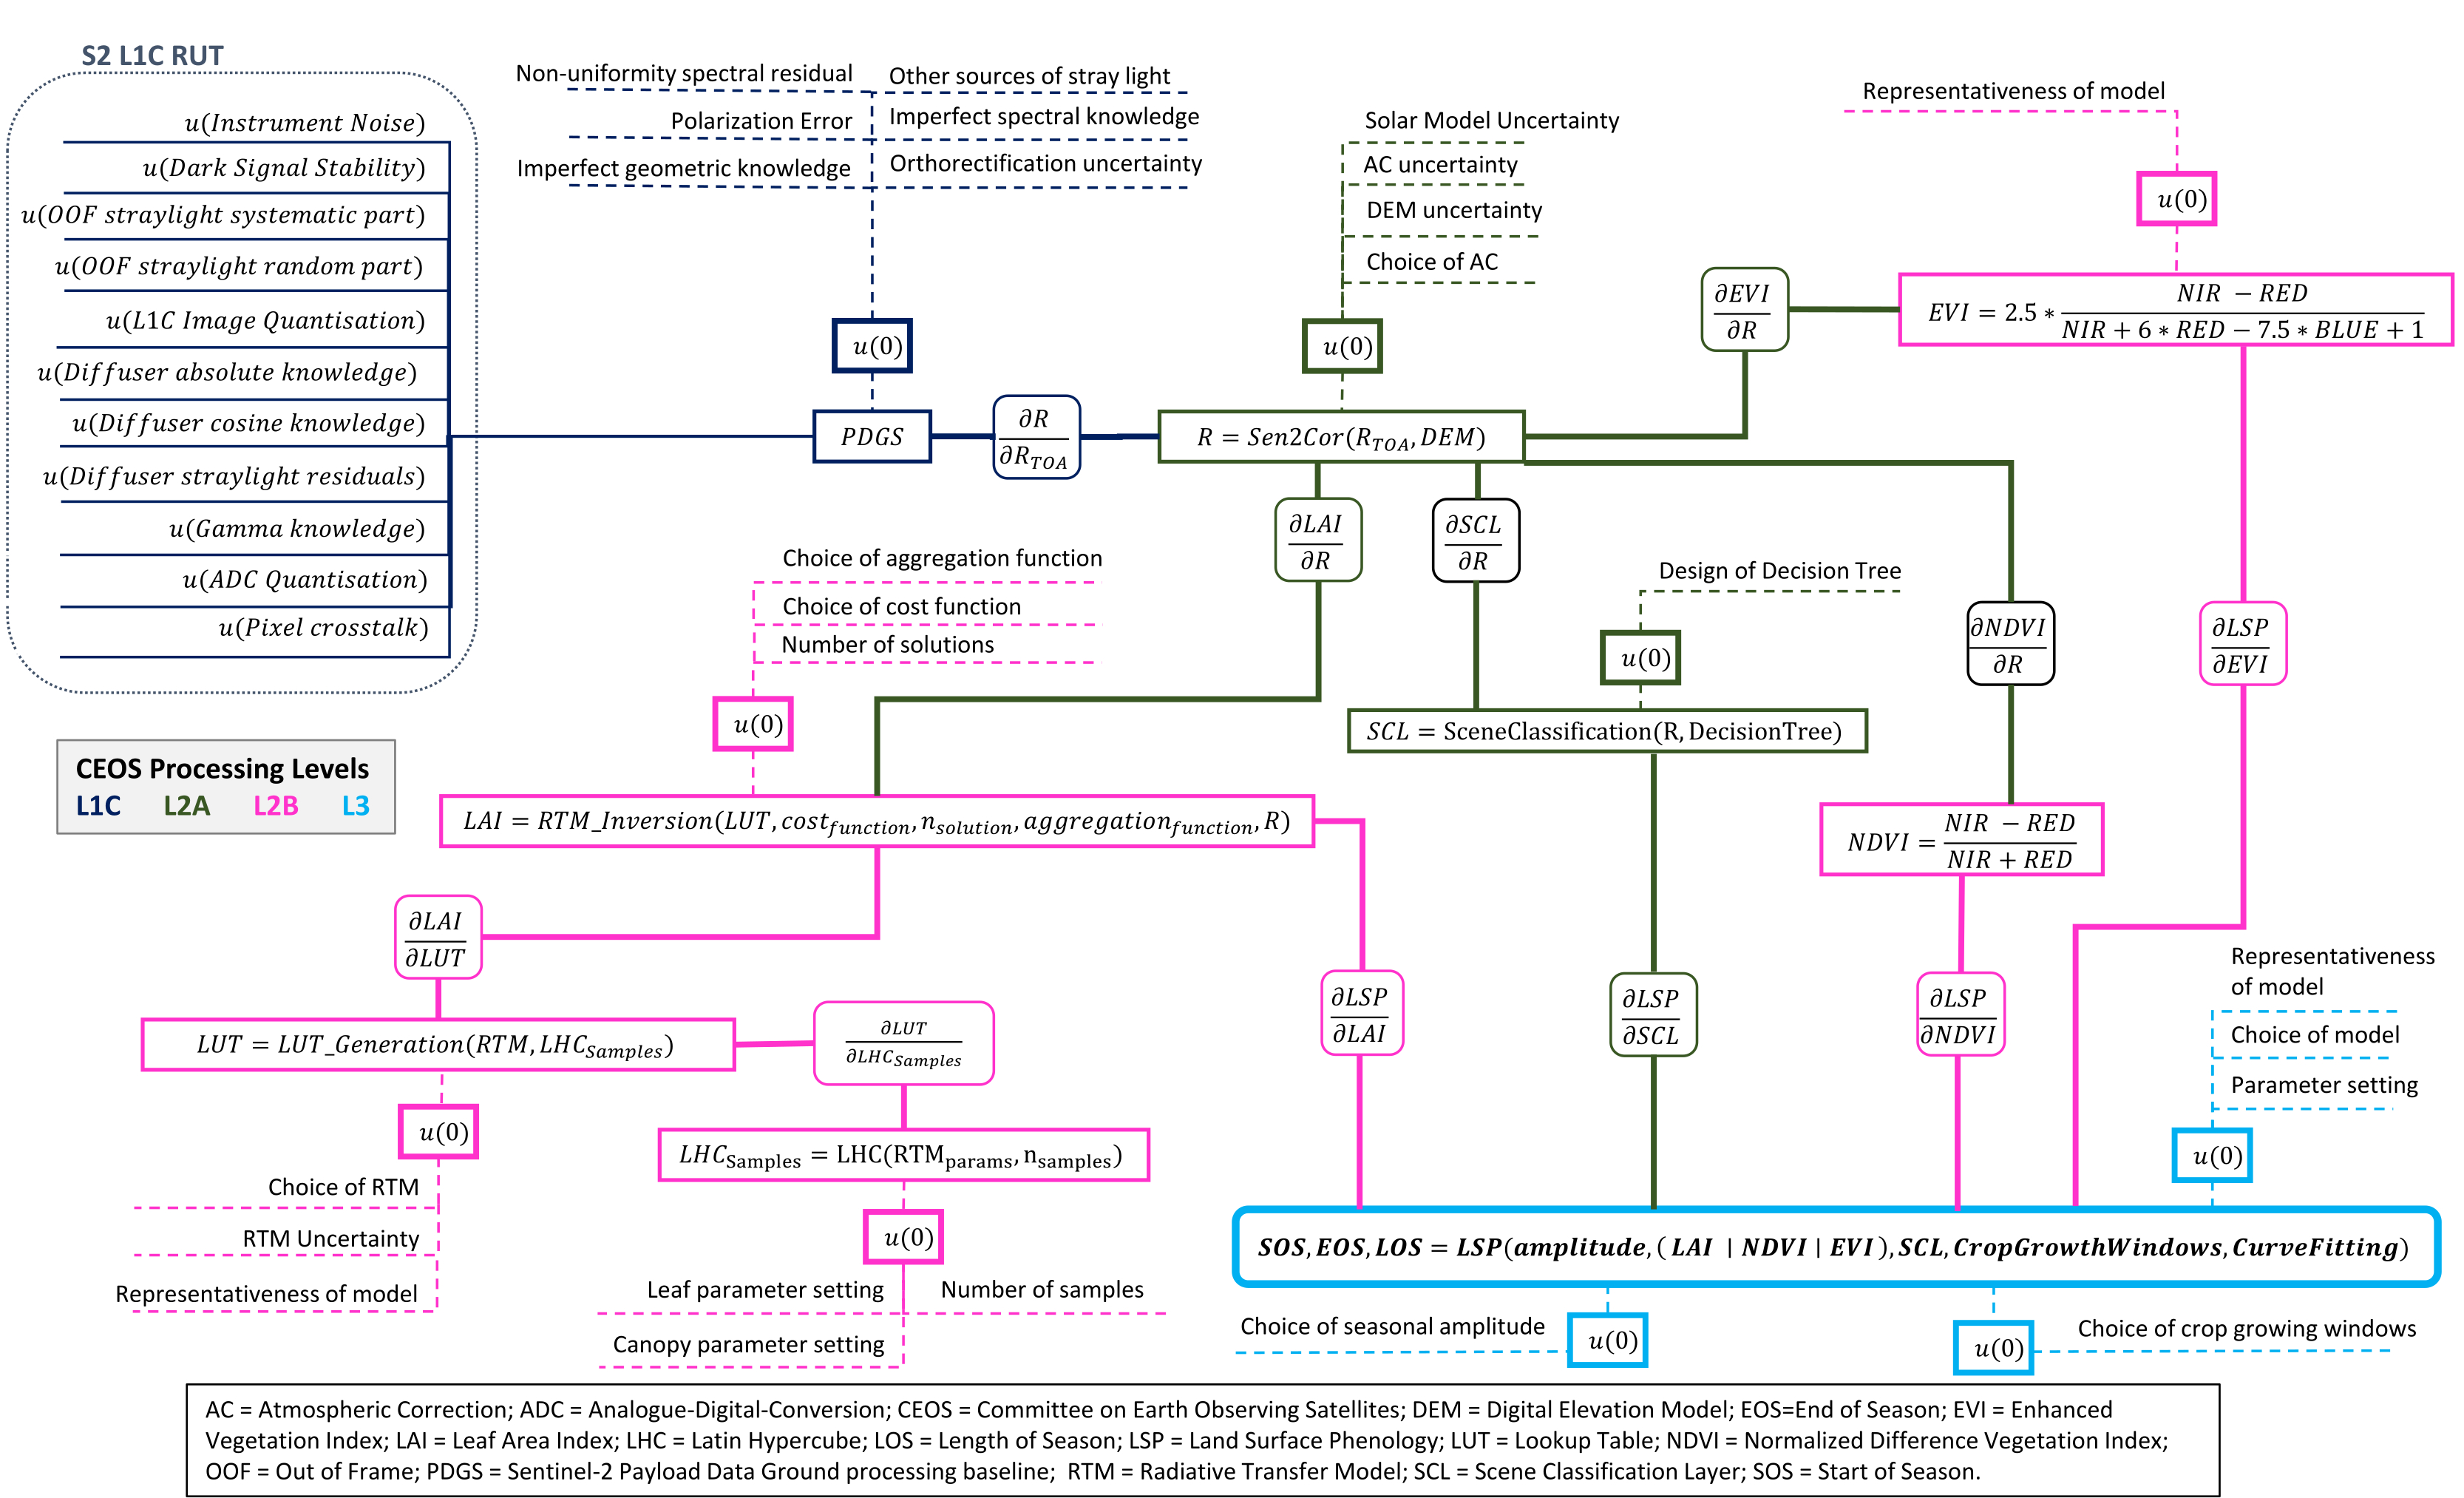
\includegraphics[angle=90, scale=0.6]{uncertainty_diagram_updated.jpg}
    \caption{Uncertainty tree diagram of uncertainty in \gls{LSP} metrics derived from multi-temporal \gls{S2} data (blue box). Processing levels defined by the Committee on Earth Observing Satellites (CEOS) are color-coded starting at L1C (dark blue) and ending at the \gls{LSP} metrics (L3). Partial derivatives represent sensitivity coefficients showing how uncertainty propagates from certain source effects into the end product. Uncertainty contributors not considered in this study are indicated by $\mu(0)$.}
    \label{fig:unc-diagram}
\end{figure*}


\subsection{S2 Radiometric Uncertainty}
\label{subsec:s2-rut}
We calculated the pixel-based uncertainty in the \gls{S2} \gls{TOA}reflectance factor values using the \gls{S2-RUT} which is an extension to the Sentinels Application Platform (SNAP). The \gls{S2-RUT} takes a \gls{S2} L1C product as input and returns the relative standard uncertainty of each implemented contributor for each pixel in each spectral band in its native spatial resolution (Figure \ref{fig:figure2-workflow}a). Overall, 11 uncertainty contributors were considered (see Figure \ref{fig:unc-diagram}, dashed box in the top left corner) based on \cite{gorrono_providing_2018}. Other sources of error in the PDGS process chain, at the end of which is the L1C product, were not considered, such as polarization error (denoted by $\mu(0)$ above the ``PDGS'' box in Figure \ref{fig:unc-diagram}). For a detailed explanation of the error sources used in the S2-RUT, as well as the effects of those not considered, the reader is referred to \cite{gorrono_radiometric_2017} and \cite{gorrono_providing_2018}. 

\subsection{Monte Carlo Simulation of \gls{S2} \gls{TOA} Reflectance Factors}
\label{subsec:mc_sim_l1c}

To convert the radiometric uncertainty obtained per spectral band and contributor from the \gls{S2-RUT} into higher level products, we implemented a \gls{MC} framework for error propagation working on single \gls{S2} scenes (Figure \ref{fig:figure2-workflow}a). The goal is to generate L1C \gls{TOA}reflectance factor scenarios from random samples, which include the determined radiometric uncertainty and the known error correlations in the spectral, spatial and temporal domains. The domains differ in their definition from the common remote sensing terminology, except for the spectral domain. The spatial component comprises the pixels along a scan line of the \gls{MSI} detector array. This domain corresponds to the across-flight direction which is approximately E-W direction. The temporal domain, in turn, denotes consecutively scanned lines along the sensor flight direction, i.e., approximately N-S direction (see also Section \ref{sec:terms-and-definitions}).

The MC-derived error in a single pixel $i$ from uncertainty contributor $j$ in \gls{MC} iteration (scenario) $t$ ($\delta_{t,j,i}$) is a linear combination of uncorrelated ($\delta_{ucorr\_i}$) and correlated ($\delta_{corr\_i}$) error terms:

\begin{equation}
    \label{eq:unc_corr}
    \delta_{t,j,i} = (1-\alpha) \cdot \mu_{j,i}^{RUT} \cdot x_{t,j,i}^{ucorr} + \alpha \cdot \mu_{j,i}^{RUT} * x_{t,j}^{corr}
\end{equation}

The left-hand side of Equation \ref{eq:unc_corr} denotes the uncorrelated error term, where $\mu_{j,i}^{RUT}$ is the pixel-based uncorrelated radiometric uncertainty (see \ref{subsec:s2-rut}) and $x_{t,j,i}^{ucorr}$ is a sample drawn from a Gaussian $\mathcal{N}(0,1)$ or uniform $U(-1,1)$ distribution for each contributor $j$. The right-hand side denotes the correlated error term where a single sample $x_{t,j}$ is drawn for all pixels and scaled by the \gls{S2-RUT} derived uncertainty. The correlation coefficient $\alpha$ takes values between 0 and 1, where $\alpha = 0$ means that the error is completely independent. When $\alpha$ is 1, then an error is fully correlated between pixels and spectral bands. The values for $\alpha$ within the three domains for the single uncertainty contributors are based on correlation coefficients reported by \cite[Table 1]{gorrono_providing_2018}.

While the  \gls{MC} framework is rather easy to implement, a sufficiently high number of realisations (scenarios) is essential to obtain reliable results. Running Sen2Cor on a single scene took approximately 15 minutes on a powerful workstation running under Linux Fedora 34 (16 Core AMD Ryzen Threadripper PRO 3955WX 3.9GHz, 128GB DDR4 3200MHz, SSD drives). To determine the necessary number of scenarios in the  \gls{MC} framework, we selected three \gls{S2} scenes at different times of the year and created 1000 L1C scenarios for each of the scenes using the aforementioned  \gls{MC} framework. Then we applied the image processing chain (see Section \ref{sec:sentinel2-processing-chain}). Next, we calculated the uncertainty in each of these variables. We started calculating the uncertainty using two scenarios and iteratively increased the number of scenarios up to 1000. Then, we plotted the retrieved absolute uncertainty values (per target variable and different crop types) against the number of scenarios considered. We determined a number of 300 scenarios as an optimum threshold after which the derived uncertainty converged against a fixed value.

\subsection{Sentinel-2 Processing Chain}
\label{sec:sentinel2-processing-chain}
Each L1C \gls{TOA} scenario is processed using a classical remote sensing image processing, which underlies most \gls{LSP} studies. First, atmospheric correction is performed to minimize atmospheric influences. The atmospheric-corrected data are then used in a second step to determine NDVI, EVI, and the \gls{GLAI} (\ref{fig:figure2-workflow}a). The standard deviation of these across all scenarios of an \gls{S2} scene gives its standard uncertainty ($k=1$). This is determined from all scenes and used to generate time series scenarios from which the \gls{LSP} metrics are calculated. Besides atmospheric correction all processing steps were carried out using the open-source Python Earth Observation Data Analysis Library (EOdal, \citep{graf_eodal_2022}). The code required to re-run the uncertainty propagation chain and subsequent is available publicly under GNU 3.0 license\footnote{\url{https://doi.org/10.5281/zenodo.6669854}}.

\subsubsection{Atmospheric correction}
\label{subsubsec:atcor}
All scenes and their \gls{MC} scenarios in L1C processing level were converted to BOA (L2A) reflectance factors using Sen2Cor v2.9 \cite{muller-wilm_sentinel-2_2013,main-knorn_sen2cor_2017}. While there are many software packages available for atmospheric correction (AC) of Sentinel-2 scenes, we selected Sen2Cor because it is integrated by the operational Copernicus \gls{S2} ground segment and some of the DIAS platforms. Additionally, the widely-used Google Earth Engine \citep{gorelick_google_2017} platforms provides Sen2Cor-processed \gls{S2} L2A data.

Important to note, we used the default configuration of Sen2Cor for all runs. Thus, we propagated the radiometric uncertainty through the AC without introducing uncertainty of the AC itself (see Figure \ref{fig:unc-diagram}). Therefore, we do not further address the uncertainties of the AC and its parameters (water vapor, aerosol optical depth). Quantifying the uncertainty of the AC itself is a complex task far beyond the scope of this paper. Currently, a follow-up paper describing AC uncertainty quantification is in preparation by \textsc{Gorron\~o et al.} The source code is already available: \url{https://zenodo.org/record/7826096}.

\subsubsection{Uncertainty of the scene classification layer}
\label{subsubsec:slc_uncertainty}
For each L1C \gls{MC} scenario, an \gls{SCL} result is available after atmospheric correction (see \ref{subsubsec:atcor}). Again, we focus on the effect of propagated radiometric uncertainty and do not consider, e.g., the design and parametrisation of the classifier.

For each  \gls{MC} scenario of a \gls{S2} scene, the percentage of pixels belonging to one of the 12 \gls{SCL} classes was computed. Then, the mean and standard deviation across all  \gls{MC} scenarios of a scene was calculated per \gls{SCL} class giving a quantitative estimate how radiometric uncertainty influenced the number of pixels belonging to a certain class. In addition, for each pixel a confidence score $C_i$ was provided for the \gls{SCL} class $i$ the majority of the  \gls{MC} runs ($N=300$) voted for. A confidence score of $100\%$ for \gls{SCL} class $i$ of a pixel indicates that all $N$  \gls{MC} scenarios had the same \gls{SCL} class whereas lower percentages indicate that a certain share of $j$ ($0 \le j \le N$)  \gls{MC} scenarios resulted in different \gls{SCL} classification outputs:

\begin{equation}
    \label{eq:confidence-score}
    C_i = \frac{N-j}{N}
\end{equation}

\subsubsection{Vegetation Indices and Parameters}
\label{subsubsec:vis_and_params}
\label{subsubsec:vis_params}
Using the Sen2Cor derived L2A BOA reflectance factors we calculated two widely used spectral vegetation indices (VI), which were recently reported to have been used in more than 80\% of 445 \gls{LSP} studies \citep{caparros-santiago_land_2021}. Using the \gls{SCL} product, pixels were masked if not classified as Class 4 (vegetation), or 5 (non-vegetated, linked to bare soil and brown vegetation).

The most common index is the \gls{NDVI} \citep{rouse_monitoring_1974} which is sensitive to canopy greenness. We calculated the \gls{NDVI} using \gls{S2} bands B04 (red) and B08 (near-infrared) which both have a spatial resolution of 10 m.

\begin{equation}
\label{eq:ndvi}
NDVI  = \frac{B08 - B04}{B08 + B04}
\end{equation}

Additionally, we calculated the three-band \gls{EVI} \citep{huete_overview_2002} that utilizes the blue band (B02) in addition (spatial resolution $10$ m). In contrast to the NDVI, the \gls{EVI} is less prone to saturation effects for high biomass values and has reduced sensitivity to background and atmospheric effects. However, this comes at the price of empirical coefficients, which are an additional source of uncertainty (see Figure \ref{fig:unc-diagram}, denoted as ``representativeness of model``).

\begin{equation}
\label{eq:evi}
EVI  = 2.5 \frac{B08-B04}{B08 + 6B04 - 7.5B02 + 1}
\end{equation}

Both, \gls{NDVI} and \gls{EVI} are canopy greenness proxies whose development is linked to changes in plant physiology \citep{bolton_continental-scale_2020,kamenova_evaluation_2021}. \gls{NDVI} and \gls{EVI} take values between -1 and +1. The higher the value, the more green (i.e., healthy) vegetation is.

For \gls{GLAI} retrieval, we developed a \gls{LUT} based inversion approach of the four-stream RTM PROSAIL \citep{jacquemoud_prospectsail_2009} using PROSPECT-D as leaf model \citep{feret_prospect-d_2017}. We created a large \gls{LUT} for each \gls{S2} scene with 50000 entries using a latin-hyper-cube sampling scheme. The range of input leaf and canopy parameters were limited to upper and lower bounds suggested by \cite{danner_efficient_2021}. Sun and observer angles where set to scene-specific values. By comparing the PROSAIL-simulated \gls{S2} BOA spectra in the \gls{LUT} with satellite observations by means of the root-mean-squared-error (RMSE) we retrieved the LAI as the median of the 100 best-fitting solutions.

As with the previous steps in the processing chains there are further sources of uncertainty which cannot be addressed within the scope of this work: PROSAIL, for instance, has an inherent uncertainty, while the size of the \gls{LUT} as well as the underlying sampling strategy most likely have an influence on the inversion result like the inversion strategy itself. Likewise, another RTM could have been used instead of PROSAIL. These effects are denoted with $\mu(0)$ in Figure \ref{fig:unc-diagram}.

\subsubsection{Time Series Generation and Phenology Extraction}
\label{subsubsec:time-series}

For each crop, growing periods were defined based on agronomic knowledge, since the period studied (February to October) is longer than the growing period of most of the crops considered. For example, winter wheat and barley are harvested in Switzerland by mid to late July at the latest, whereas maize or soybean are not sown before mid-April. Therefore, \gls{S2} observations before or after the main crop growth period were discarded. Table \ref{tab:crop-periods} shows the chosen crop growing periods for all crop types available. In addition to agronomic knowledge, start and end dates were adjusted manually based on Sentinel-2 data availability (see Figure \ref{fig:s2-scenes}) to ensure that sufficient data points were available at the beginning and end of the growing season.

\begin{table*}
\centering
\caption{Key crop growth periods defined based on agronomic knowledge to constrain the temporal range considered per crop type between a start and end date (YYYY-MM-DD).}
\begin{tabular*}{\textwidth}{@{\extracolsep{\fill}}rcr}
Crop Type                     & Start      & End        \\
\hline
Winter Wheat              & 2019-02-01 & 2019-08-15 \\
Winter Barley             & 2019-02-01 & 2019-08-15 \\
Grain Maize               & 2019-05-01 & 2019-10-15 \\
Silage Maize              & 2019-05-01 & 2019-10-15 \\
Soybean                   & 2019-04-01 & 2019-10-15 \\
Potato                    & 2019-04-01 & 2019-10-15 \\
Rapeseed                  & 2019-02-01 & 2019-08-15 \\
Permanent Grassland        & 2019-02-01 & 2019-10-15 \\
Extensively Used Grassland & 2019-02-01 & 2019-10-15 \\
Sugar Beet                & 2019-04-01 & 2019-10-15 \\
Sunflower                 & 2019-04-01 & 2019-10-15 \\
\hline
\end{tabular*}
\label{tab:crop-periods}
\end{table*}

For the time series analysis, an approach based on the widely used TIMESAT software \citep{eklundh_timesat_2015} (v3.3) was chosen, which ensures the comparability of this work with other \gls{LSP} studies (Figure \ref{fig:figure2-workflow}b). We used the Python package ``phenolopy'' available under Apache-2.0 license that implements the TIMESAT v3.3 approach in Python \citep{trotter_frontiersiphenolopy_2021}. Subsequently, a simple outlier detection was performed with a moving median with a window width of five subsequent observations. Data points that deviate more than the user-defined cutoff value from the median of the window and are also smaller than the mean of the immediate two neighbors minus the cutoff value are identified as outliers. In this case, the cutoff value was set to two standard deviations. The remaining data points were interpolated linearly to obtain daily values. The outlier removal was applied after filtering by SCL. Overall, the number of outliers can be considered low ($\le10$\% of all data points), since mainly cloud-free scenes were used. In a further step, the time series was smoothed with a Savitzky-Golay filter \citep{savitzky_smoothing_1964}, using a window size of 11 days and a first degree polynomial. Savitzky-Golay is a widely used method in remote sensing studies for smoothing time series \citep{chen_simple_2004,zhou_performance_2016,de_castro_mapping_2018}. Again, the uncertainty arising from the outlier removal and curve fitting is denoted with $\mu(0)$ (Figure \ref{fig:unc-diagram}).

The \gls{LSP} metrics \gls{SOS} and \gls{EOS} were calculated using a 20\% threshold in seasonal amplitude. The seasonal amplitude is defined as the difference between the maximum value of the time series and a base-line. The base-line is given by the mean value of the minimum before and after the maximum of the time series. The \gls{SOS} is the date when the time series reaches 20\% of the amplitude and the end of season is the date when the time series falls below this value after the maximum for the first time \citep{jonsson_seasonality_2003, caparros-santiago_land_2021}. The \gls{LOS} can be calculated as the difference between the timing of \gls{SOS} and \gls{EOS} in days. Of course, the choice of seasonal amplitude is also a source of uncertainty which we set to zero in this study (Figure \ref{fig:unc-diagram}).

Figure \ref{fig:lsp_example} exemplifies the concept of the seasonal amplitude for a single sunflower pixel in the study area. The blue dots denote the raw \gls{GLAI} values derived from ProSAIL whereas the blue solid line shows the result after outlier removal and smoothing using Savitzky-Golay in daily resolution.

\begin{figure*}
    \centering
    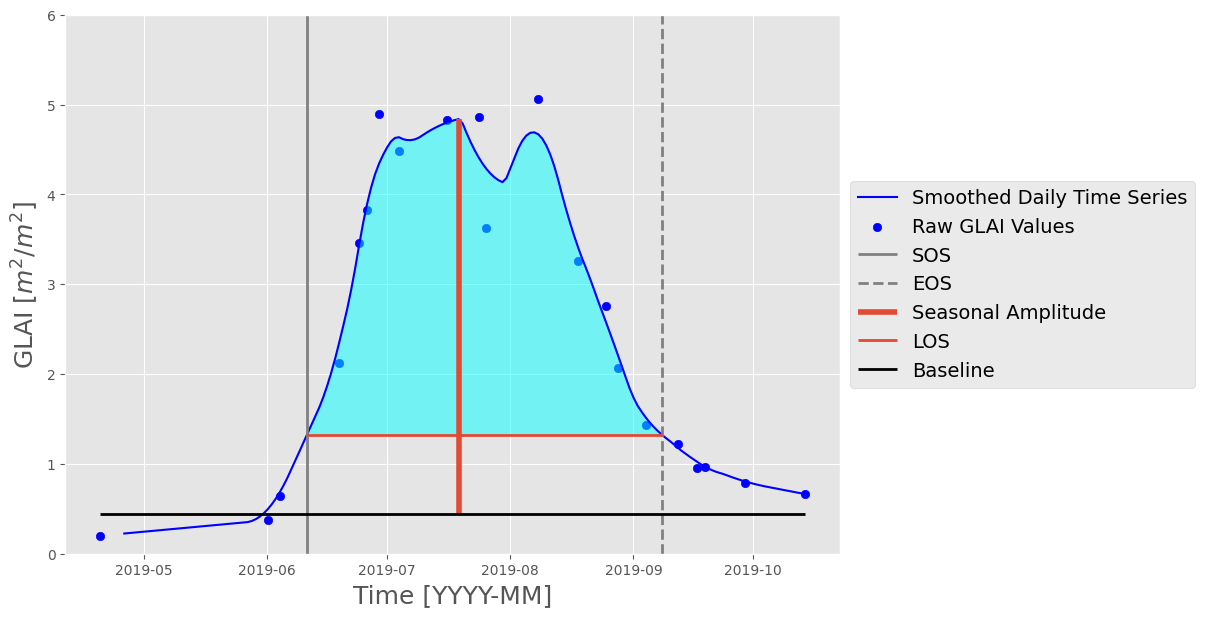
\includegraphics[width=1.0\textwidth]{lsp_sample_time_series.png}
    \caption{Example \gls{GLAI} time series from a single pixel in daily resolution (blue solid line) derived from raw \gls{GLAI} values (blue dots) showing \gls{SOS} (grey solid line), \gls{EOS} (grey dashed line), \gls{LOS} (red horizontal line) for a single sunflower pixel using a threshold of 20\% seasonal amplitude (bold vertical red line). The area colored in cyan between the \gls{GLAI} curve and the \gls{LOS} line represents the actual growing season.}
    \label{fig:lsp_example}
\end{figure*}

\subsection{Time Series Scenarios}
\label{subsec:time-series-scenarios}
The methodology described in Section \ref{subsubsec:time-series} was embedded into a second \gls{MC} framework (Figure \ref{fig:figure2-workflow}c+d) to generate time series scenarios. \gls{MC} sampling was performed to create the time series scenarios ($N=1000$) for propagating radiometric uncertainty into \gls{LSP} metrics. Pixel time series were generated using the original \gls{EVI}, \gls{NDVI} and \gls{GLAI} values and their uncertainty derived from Section \ref{subsubsec:vis_and_params}.

For scenario generation, two different types of error correlation (see also Section \ref{subsec:mc_sim_l1c}) were assumed. Since it is currently unknown to what extent systematic effects have an impact between the individual \gls{S2} scenes, two different approaches were run, reflecting the two possible extreme cases:

\begin{enumerate}
    \item Full correlation ($\alpha=1$) between the \gls{S2} scenes, i.e., the determined uncertainty in the VIs or the \gls{GLAI} affects all dates equally per pixel (Figure \ref{fig:figure2-workflow}c).
    \item  Zero inter-scene correlation ($\alpha=0$) where the single \gls{S2} scenes are completely uncorrelated and the uncertainties of the dates of a pixel are thus stochastically independent (Figure \ref{fig:figure2-workflow}d).
\end{enumerate}

Errors can be correlated due to systematic effects such as straylight during the sensor (re-)calibration. Instrument noise or analog-to-digital quantization, in turn, are uncorrelated between scenes and therefore favor the uncorrelated assumption.

\section{Results}
\label{sec:unc_results}

\subsection{Scene Classification Layer Uncertainty}
Radiometric uncertainty imposed uncertainties in \gls{SCL} class assignment. Figure \ref{fig:figure3-scl_uncertainty} shows a true color representation of the study area taken by S2A on May 30, 2019 (Figure \ref{fig:figure3-scl_uncertainty} A) and the corresponding \gls{SCL} calculated from the majority vote of all 300  \gls{MC} realizations (Figure \ref{fig:figure3-scl_uncertainty} B). Figure \ref{fig:figure3-scl_uncertainty} C shows that the \gls{SCL} class membership was mostly close or equal to 100\%, i.e., the pixel-based classification was the same in all 300 scenarios. In particular, areas with homogeneous spectral properties, such as vegetated areas, but also the central regions of the cumulus clouds and their shadows had a high confidence (100\%), thus a low classification uncertainty. At the transition area of two classes, e.g. at the transition from cloud to cloud shadow or cloud shadow to vegetation, lower confidence values (smaller than 48\% in some cases) and thus higher uncertainty due to spectral mixing effects caused by the spatial resolution of $20$ m of the \gls{SCL} product and adjacency effects were shown. This is clearly evident from the small-scale detail plot in Figure \ref{fig:figure3-scl_uncertainty}D-F. Depending on the cloudiness of a scene the relative number of pixels where the class assignment confidence was <100\% was 88.2\% (2019-05-30, cloudy pixel percentage: 17\%) to 94.6\% (2019-06-19, cloudy pixel percentage: 0.6\%).

Throughout the entire season, average class confidence was highest for vegetation ($99.3\pm0.8$\%), clouds with high probability ($96.4\pm1.7$\%), non-vegetated pixels ($95.9\pm1.7$\%), and thin cirrus ($95.6\pm3.8$\%) followed by clouds with medium probability ($92.0\pm2.3$\%). Also the water ($95.1\pm1.8$\%), unclassified ($91\pm2.4$\%), and dark area pixel class ($93.3\pm2.2$\%) scored high on average. These classes, however, were less abundant in the \gls{S2} scenes (see, for instance, Figure \ref{fig:figure3-scl_uncertainty}). Cloud shadows ($84.9\pm2.6$\%) had the lowest average confidence score.

\begin{figure*}
    \centering
    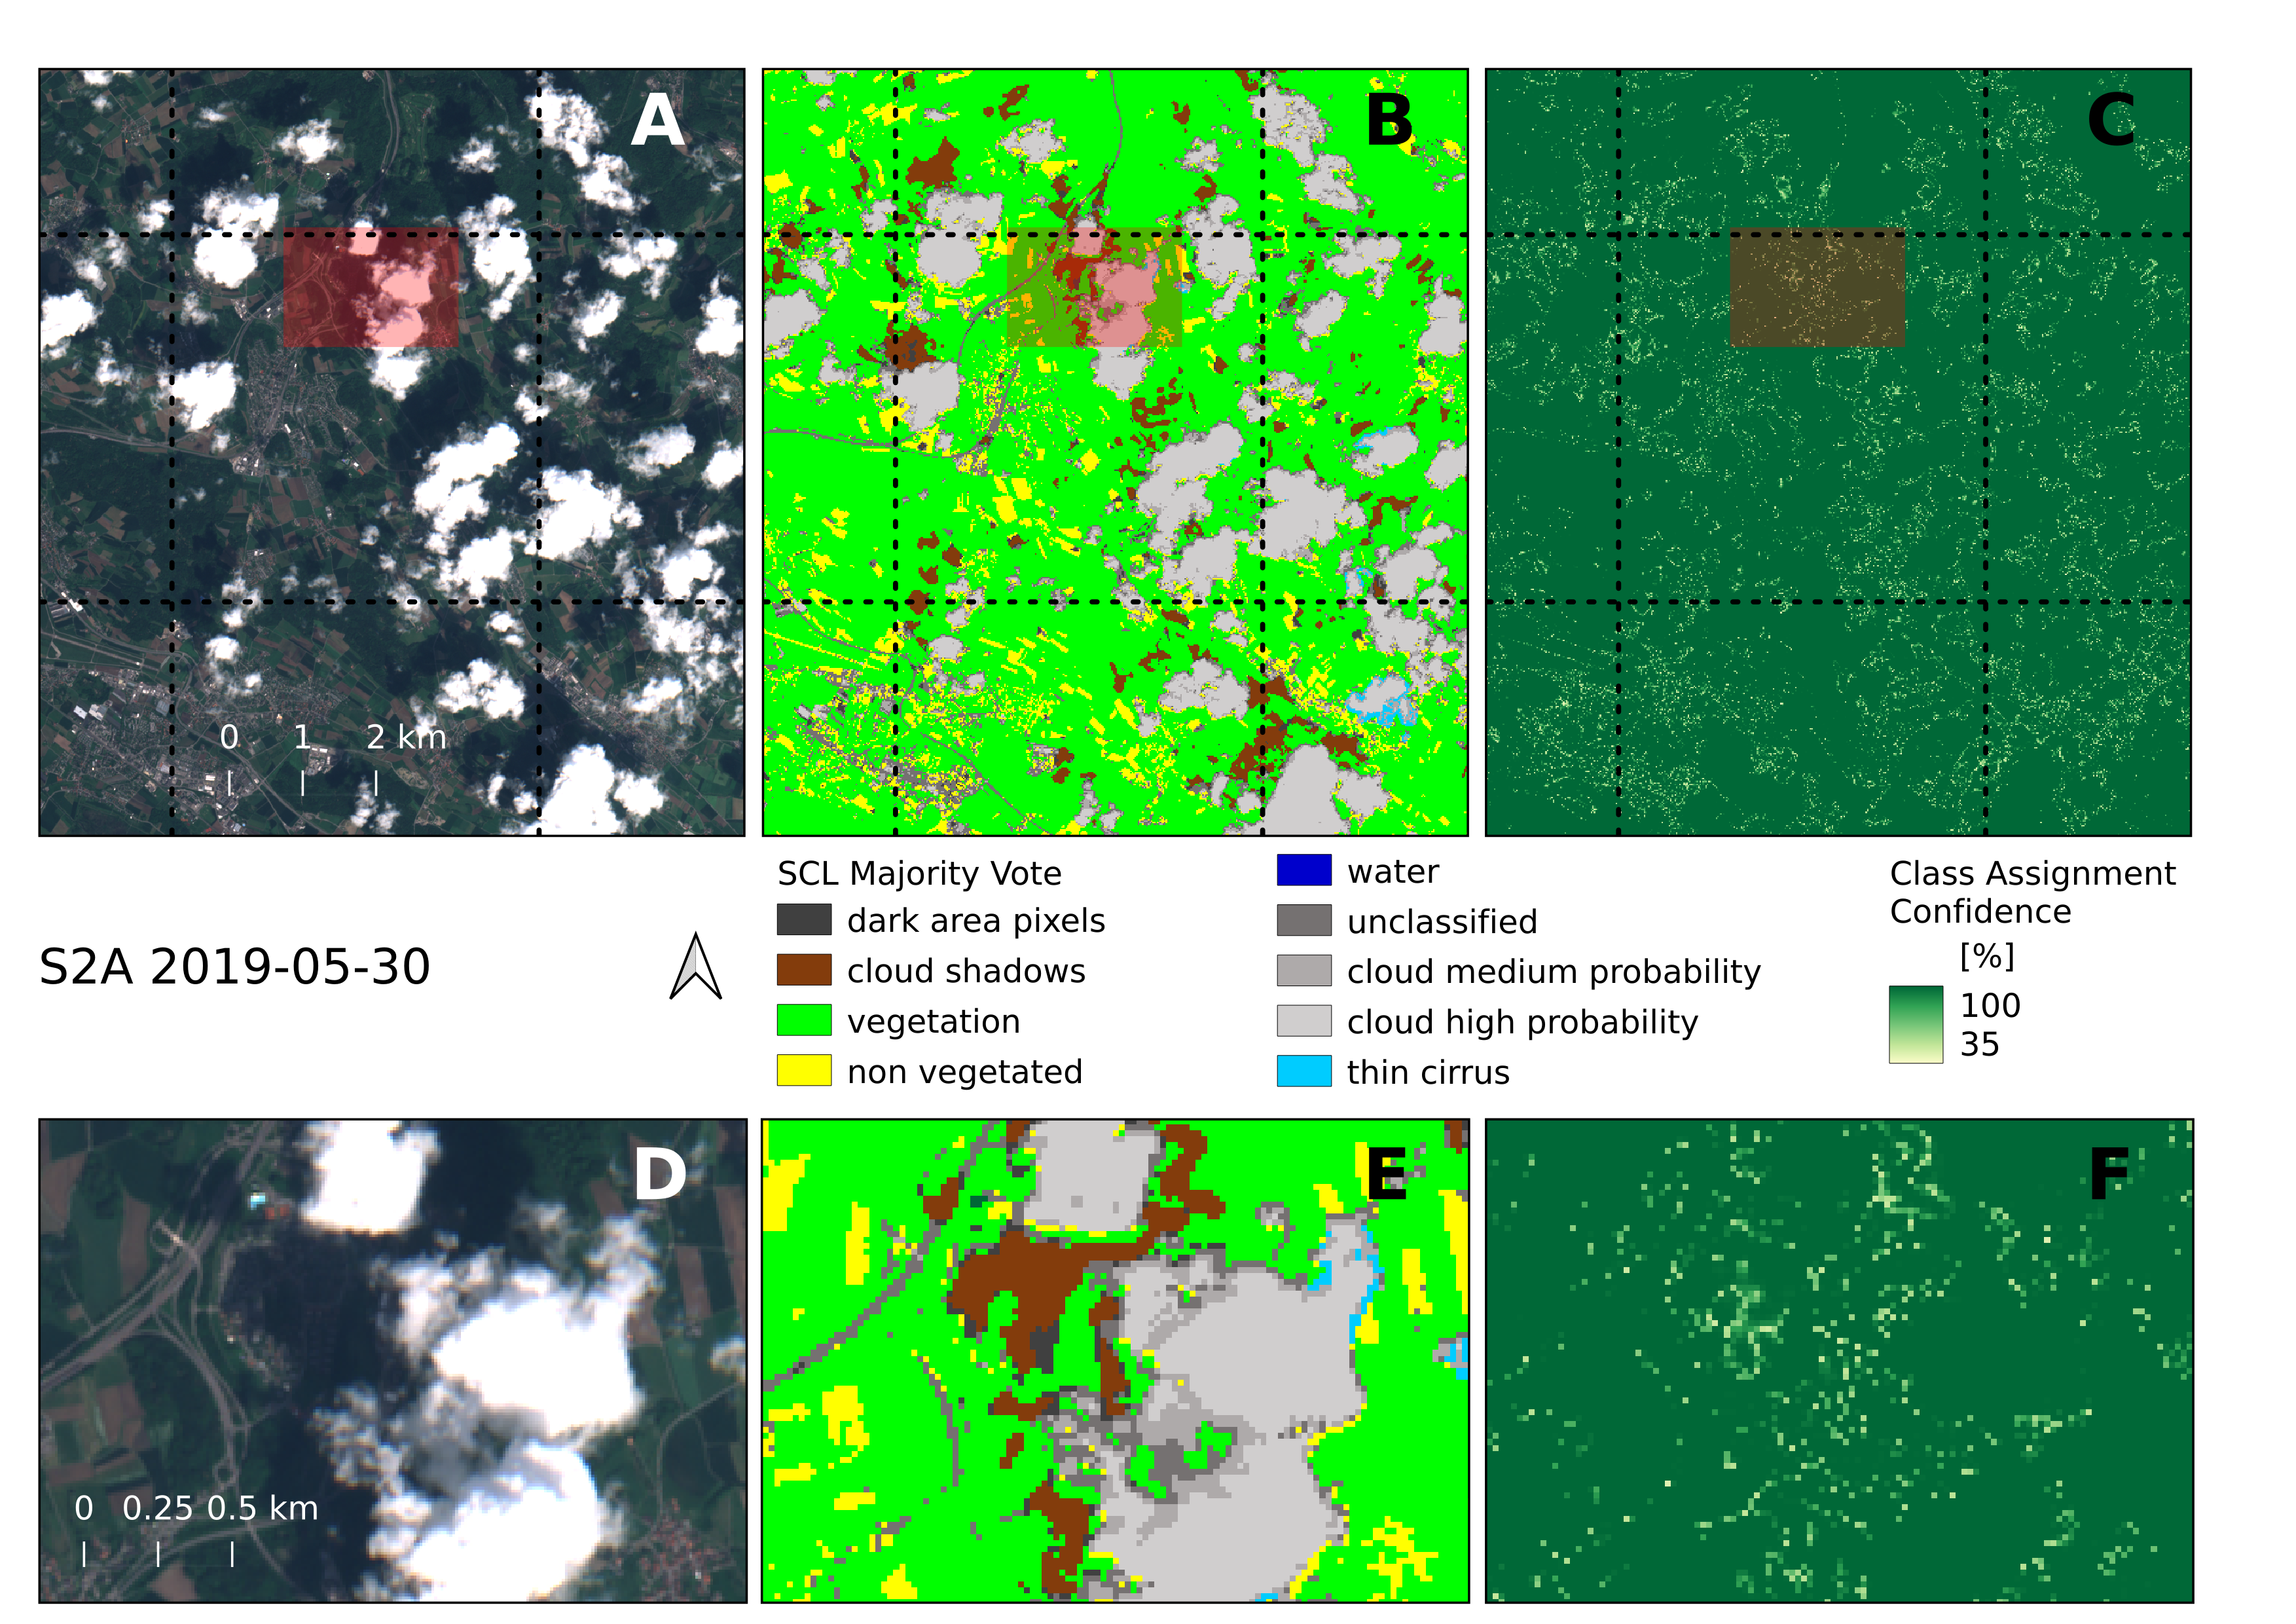
\includegraphics[width=1.0\textwidth]{Figure_3-SCL uncertainty.png}
    \caption{RGB L1C \gls{TOA}true-color composite (A), \gls{SCL} majority vote (B) and \gls{SCL} class assignment confidence scores (C) for a S2A scene acquired on May 30th 2019. The more greenish the color in C the higher the confidence score and the lower the uncertainty. A small-scale detail plot (red rectangle in A-C) highlighting the higher uncertainties at class boundaries is depicted in D to F.}
    \label{fig:figure3-scl_uncertainty}
\end{figure*}

Looking at the relative uncertainty in the percentage of pixels (\%) assigned to an \gls{SCL} class per \gls{S2} scene, we noted cloud classes (medium and high probability) to have a higher relative uncertainty of up to 4\% than vegetation ($\le0.1\%$) and bare-soil ($\le1.5\%$). Table \ref{tab:scl-uncertainty} shows the uncertainty in the relative number of pixels per class in relation to all \gls{S2} pixels (360000 pixels, 20 m spatial resolution) for five selected scenes including the scene from May 30th (Figure \ref{fig:figure3-scl_uncertainty}). The complete table can be found in Table \ref{supp:scl_uncertainty}. The scenes were selected to represent different important times in vegetation development, such as the end of winter dormancy, advanced spring, early and mid-summer, and incipient fall. Pixels from one of the two cloud classes often only change from medium to high cloud probability and vice versa, whereas vegetation pixels are classified as cloud shadows in some scenarios. This is significant because unrecognized cloud shadows are among the main causes of outliers in vegetation time series.

\begin{table*}
\caption{Mean percentage of pixels for selected \gls{SCL} classes $\pm$ standard deviation derived from 300  \gls{MC} realizations for five \gls{S2} scenes. The overall number of pixels per scene is 360000 (20 $\times$ 20 m spatial resolution). The complete table including all \gls{SCL} classes and \gls{S2} scenes can be found in Table \ref{supp:scl_uncertainty} in the supplementary materials.}
\label{tab:scl-uncertainty}
\begin{tabular*}{\textwidth}{@{\extracolsep{\fill}}rccccr}
\toprule
      \pbox{1cm}{sensing date} &  \pbox{1cm}{cloud shadows} &  \pbox{1cm}{vegetation} & \pbox{1cm}{non vegetated} & \pbox{1cm}{cloud medium probability} & \pbox{1cm}{cloud high probability} \\
\midrule
2019-02-14 &           $6\pm4.0$ &   $52.1\pm0.4$ &     $6.8\pm1.5$ &                    $1.0\pm4.0$ &                  $0.0\pm5.0$ \\
2019-04-20 &          $0.0\pm25.0$ & $83.3\pm0.1$ &    $13.0\pm0.6$ &                $0.4\pm3.3$ &                  $0.0\pm4.0$ \\
2019-05-30 &       $3.5\pm0.9$ & $65.2\pm0.2$ &     $7.7\pm1.0$ &                $4.3\pm1.4$ &             $12.4\pm0.4$ \\
2019-07-16 &      $2.0\pm0.8$ & $76.8\pm0.1$ &    $11.7\pm0.7$ &                $2.3\pm2.0$ &              $3.8\pm1.2$ \\
2019-09-19 & \pbox{1cm}{($0.0\pm1.1$)e+02} & $85.0\pm0.1$ &    $11.1\pm0.6$ &                $0.4\pm3.0$ &                  $0.0\pm5.0$ \\
\bottomrule
\end{tabular*}
\end{table*}


\subsection{\gls{NDVI}, \gls{EVI} and \gls{GLAI} Uncertainty}
\label{subsec:ndvi-evi-glai-uncertainty}

Figure \ref{fig:ww-rel-unc-box} shows the kernel-density based distributions of MC-derived relative uncertainty values for \gls{EVI} (left), \gls{NDVI} (middle) and \gls{GLAI} (right) per crop type (color-coded). All pixels marked as \gls{SCL} class 4 (vegetated) or 5 (non-vegetated) have been included. To improve readability the x-axis in Figure \ref{fig:ww-rel-unc-box} has been log-scaled.

Overall, \gls{NDVI} was less uncertain than EVI. The spectral indices exhibited lower relative uncertainties than \gls{GLAI}. Moreover, uncertainty distributions of \gls{EVI} and \gls{NDVI} revealed a narrow spike and delta-like shape with little dispersion while the maximum of the uncertainty distribution in \gls{GLAI} was flatter and less pronounced. The distribution of \gls{NDVI} relative uncertainties (Fig \ref{fig:ww-rel-unc-box}, middle) showed a sharp peak for all crop types between 0 and 1\%. Values greater than 10\% did not occur. Median uncertainty in \gls{NDVI} for all crops was about 1.1\% ranging between 0.8\% for permanent grassland to 2.4\% for potato. In contrast, the uncertainties in \gls{EVI} were slightly higher (Fig \ref{fig:ww-rel-unc-box}, left) as the spike was shifted in positive x direction. In detail, the maximum of the \gls{EVI} uncertainty distribution laid between 1 and 10\%. Median uncertainty in \gls{EVI} for all crops was about 2.7\%, ranging from 2.4\% for permanent grassland to 3.8\% for potato. Isolated outliers, however, assumed uncertainties larger than 10\%. \gls{GLAI} (Fig \ref{fig:ww-rel-unc-box}, right) exhibited a higher share of uncertainty values greater than 10\% while the peak of the distribution was located between 1 and 10\%. The median of the uncertainty distributions for all crops was about 4.4\% ranging from 4.1\% for extensively used grassland to 5.0\% for potato which is again the crop with highest uncertainties.

\begin{figure*}
    \centering
    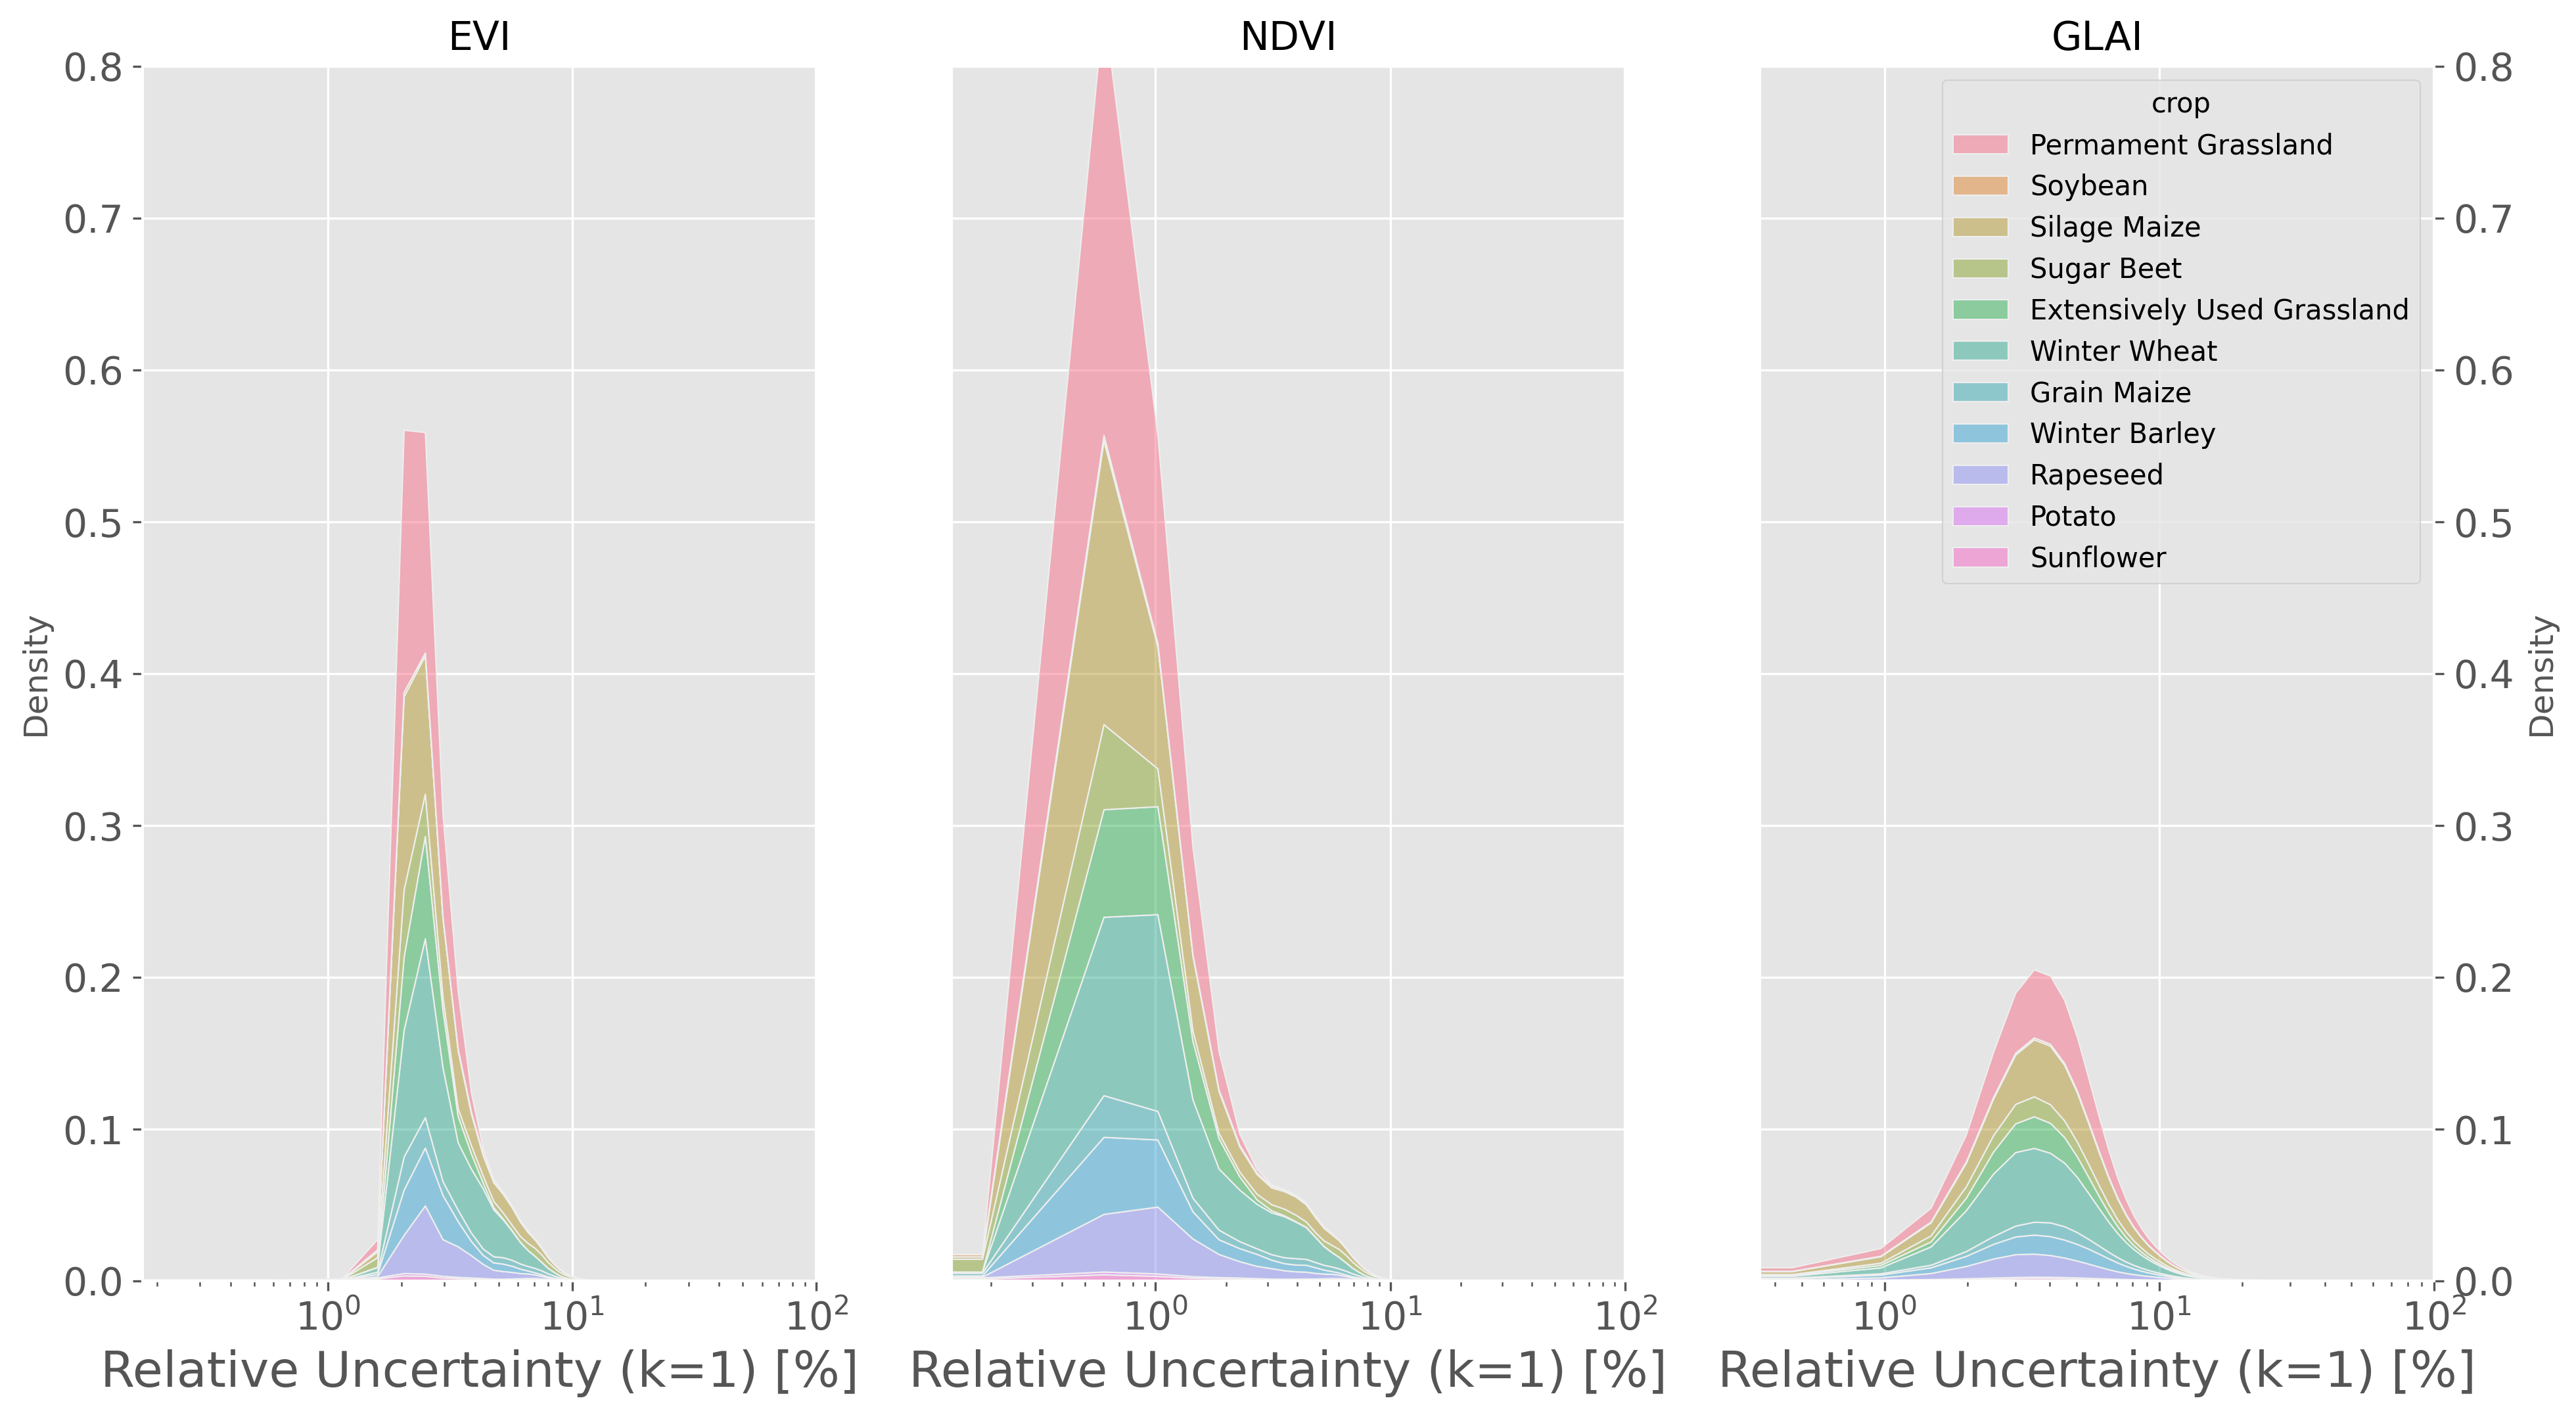
\includegraphics[width=1.0\textwidth]{vis_rel_unc_kdeplots.png}
    \caption{Kernel density based distributions of MC-derived relative uncertainty values in \gls{EVI} (left), \gls{NDVI} (middle) and \gls{GLAI} (right) considering all available crop pixels and \gls{S2} scenes excluding pixel observations not classified as "vegetated" (SCL class 4) or "non-vegetated" (SCL class 5). Contributions to relative uncertainty per crop type are color coded. To improve readability, the x-axis has been log-scaled.}
    \label{fig:ww-rel-unc-box}
\end{figure*}

For all crop types, the relative uncertainty was lowest when the canopy was greenest (high \gls{EVI} or \gls{NDVI} values) or reached the largest leaf area values (GLAI). Figure \ref{fig:ww-timeseries-and-uncertainty} showed the spatio-temporal variability in observed EVI, \gls{NDVI} and \gls{GLAI} values and their uncertainties for winter wheat (228.8 ha). In the top row in Figure \ref{fig:ww-timeseries-and-uncertainty} the median (blue line), central 50\% (red fill) and central 90\% percentile (orange) of all pixels not classified as cloud, cirrus, cloud shadow or snow was shown for each \gls{S2} scene. In the same way the  \gls{MC} derived absolute uncertainties were displayed in the mid-row of Figure \ref{fig:ww-timeseries-and-uncertainty} alongside relative uncertainty values in the bottom row. Plots for the other crops were available in the supplementary materials (Figures \ref{fig:rapeseed-timeseries-and-uncertainty}-\ref{fig:winter-barley-timeseries-and-uncertainty}) as well as pixel time series from randomly selected pixels (Figure \ref{fig:sample_ts_pixels}).

\begin{figure*}
    \centering
    \includegraphics[width=1.0\textwidth]{Fig_Winter Wheat_all-pixel-timeseries.png}
    \caption{Spatio-temporal variability of \gls{EVI} (left column), \gls{NDVI} (mid column) and \gls{GLAI} (right column) for all pixels annotated as winter wheat (228.8 ha). For each \gls{S2} scene, the median value (blue line), central 50\% (red) and 90\% spread (orange) across all pixels is shown not classified as cloud, shadow or snow based on the \gls{SCL} data of the original \gls{S2} outputs after Sen2Cor. The top-row shows the spatio-temporal variability in the actual EVI, \gls{NDVI} and \gls{GLAI} derived from the \gls{S2} scenes. In the mid row, the absolute uncertainties derived from the  \gls{MC} simulations are depicted. The bottom row shows the uncertainties in relative terms.}
    \label{fig:ww-timeseries-and-uncertainty}
\end{figure*}

Throughout the growing season, median \gls{EVI} (Figure \ref{fig:ww-timeseries-and-uncertainty}, upper left) showed a moderate increase through spring until maximum \gls{EVI} values were reached in early June. This increase was followed by a steeper decline to median \gls{EVI} values below 0.2 at the end of July. Subsequently, the median \gls{EVI} increased again. A similar picture was shown in median \gls{NDVI} (Figure \ref{fig:ww-timeseries-and-uncertainty}, top center), which started with higher values (between 0.7 and 0.5) and remained almost constant at a high level (median \gls{NDVI} > 0.8) indicating saturation between mid-April and the end of June. \gls{GLAI} (Figure \ref{fig:ww-timeseries-and-uncertainty}, upper right) showed low values at the beginning of the growth period (median \gls{GLAI} around 1 $m^2$ $m^{-2}$) and a maximum (4.5  $m^2$ $m^{-2}$) at the beginning of June. The gradient before and after this maximum was more symmetrical than for \gls{EVI} and NDVI.

Absolute uncertainties of the winter wheat pixels (Figure \ref{fig:ww-timeseries-and-uncertainty}, middle row) showed a temporal pattern, which partly reflected vegetation development. In the case of \gls{EVI} (left), the absolute uncertainties decreased first and increased moderately until the end of June (median uncertainty at the beginning of June about 0.019). Consistent with the \gls{EVI} values, the uncertainty reached a minimum at the end of July (median about 0.0075) and then increased again. In \gls{NDVI} (middle) absolute uncertainties decreased steadily, reaching a minimum in early June (median uncertainty around 0.005) and then increasing again, reaching lower values than at the beginning of the growing season (around 0.009). \gls{GLAI} (right) showed a different behavior: The absolute uncertainty curve increased similarly to the median \gls{GLAI} values from 0.05  $m^2$ $m^{-2}$ in February to the beginning of June (around 0.17  $m^2$ $m^{-2}$ median uncertainty) and then decreased to values lower than 0.05  $m^2$ $m^{-2}$ in August. From September on-wards, the uncertainties increased again. The spatial variability of the absolute uncertainties was also variable over time. Moreover, the spatial variability in absolute uncertainty was lowest in \gls{NDVI} and EVI, followed by GLAI.

Relative uncertainties (Figure \ref{fig:ww-timeseries-and-uncertainty}, bottom row) were lowest in NDVI, followed by EVI. Regarding NDVI, the median relative uncertainty was constantly below 5\% and reached the 1\% mark at the end of May. At this stage, the \gls{S2} band B08 dominated the ratio (see Eqs. \ref{eq:ndvi} and \ref{eq:evi}). The spatial variability of the relative uncertainty of \gls{NDVI} was largest at the beginning of the growth period (February to the end of March), and declined to less than one percent until the beginning of July. The spatio-temporal pattern of relative uncertainty in \gls{EVI} was similar, but relative uncertainties were higher on median than in \gls{NDVI} and exceeded the 5\% mark in August. In GLAI, the relative uncertainties were consistently higher than in the spectral indices and median values were around the 5\% mark. The spatio-temporal pattern was less evident in \gls{GLAI} than in the spectral indices and did not show a clear decrease as the growth period progresses.

\subsection{LSP Metrics Uncertainty}
\label{subsec:lsp-metrics}
\subsubsection{Start of Season}

Relative standard uncertainties distributions for \gls{SOS} are shown in Figure \ref{fig:sos-uncertainty} color-coded by crop type. The top row denotes the results when the inter-scene correlation is set to $\alpha=0$, whereas the bottom row shows the results for full inter-scene correlation ($\alpha=1$). Overall, the assumption of zero inter-scene correlations causes \gls{SOS} uncertainties to be clearly higher and more dispersed than in the case of full inter-scene correlation.

In zero inter-scene correlation (Figure \ref{fig:sos-uncertainty}, top row) the uncertainty distributions showed two distinct properties for all crop types and time series sources. First, the uncertainty distributions showed a peak shifted from zero in the magnitude of two to five days. Median uncertainties ranged from one (\gls{NDVI}  in Soybean and \gls{GLAI} in Potato) to eight days (\gls{EVI}  in rapeseed and sunflower). Second, a secondary, although less pronounced, peak with a maximum around 60 days was apparent in all three plots. In contrast to the more pronounced main peak, which had a steep right flank, the secondary peak had very flat shoulders that taper off to uncertainties of 80 days and greater.

In full inter-scene correlation (Figure \ref{fig:sos-uncertainty}, bottom row), only a single peak at 0 was evident, which was accompanied by a very steep right slope. The median uncertainty was less than one day except for the grasslands and sunflower in the GLAI, where the median was one day. 95\% of all uncertainty values were between 24 days (\gls{EVI}  in potato) and 59 days (\gls{NDVI}  in extensive grassland, winter wheat and silage maize). The second peak, which was evident in the uncorrelated case, was also evident here, although it was much less pronounced and had a maximum between 40 and 50 days.

\begin{figure*}
    \centering
    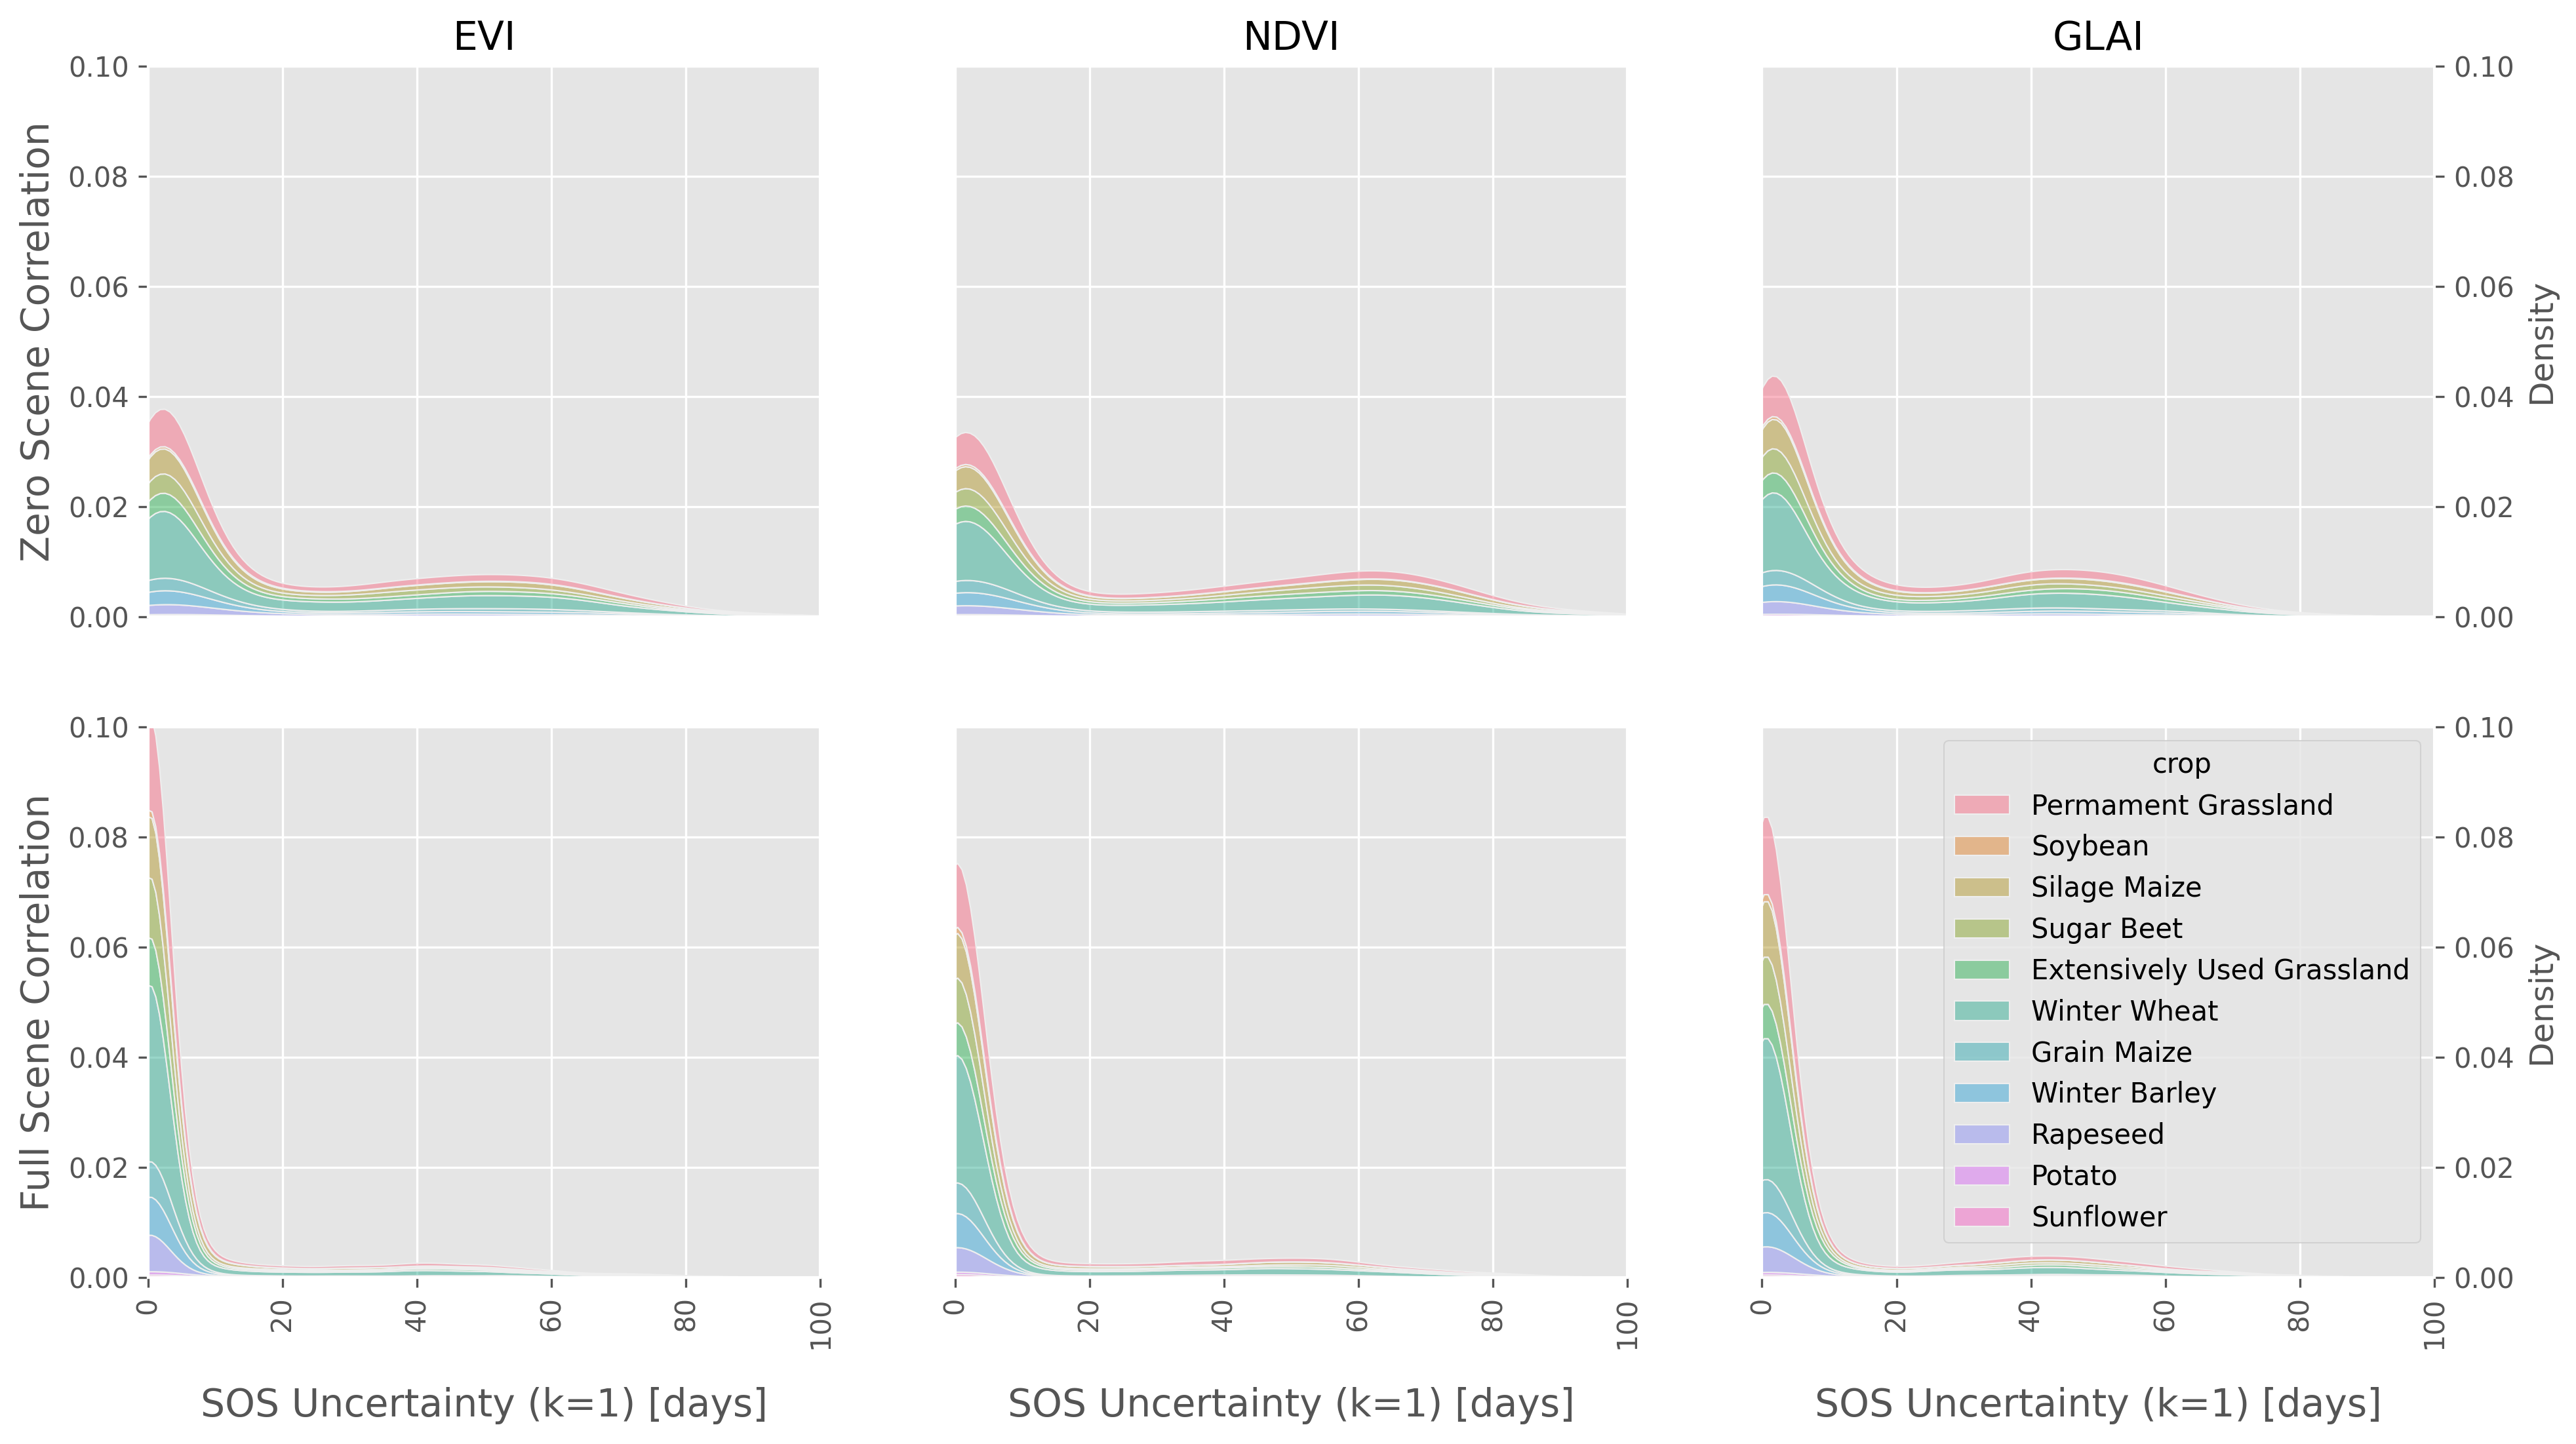
\includegraphics[width=1.0\textwidth]{sos_times_uncertainty.png}
    \caption{Kernel-based relative uncertainty distributions in Start of Season (SOS) for \gls{EVI} (left column), \gls{NDVI} (middle column), and \gls{GLAI} (right column) color-coded by crop-type. The top row shows the results of the  \gls{MC} runs with zero inter-scene correlation; the bottom row the results assuming full inter-scene correlation.}
    \label{fig:sos-uncertainty}
\end{figure*}

\subsubsection{End of Season}

Analogous to SOS, the propagated uncertainty in \gls{EOS} is shown in Figure \ref{fig:eos-uncertainty}. As for SOS, the uncertainty in the fully correlated case (Fig \ref{fig:eos-uncertainty}, bottom row) was clearly smaller than in the uncorrelated case (Fig \ref{fig:eos-uncertainty}, top row).

The uncertainty distribution in the uncorrelated case (Figure \ref{fig:eos-uncertainty}, upper row) showed a singular peak, which had a maximum between two and 20 days depending on crop type and time series source. The median uncertainty varied between two days (\gls{GLAI} in winter barley) and 16 days (\gls{EVI}  in soybean). The secondary peak evident in \gls{SOS} (see Figure \ref{fig:sos-uncertainty}) was not present. It follows that 95\% of the uncertainty values ranged from 45 days (\gls{GLAI} in sunflower) to 101 days (\gls{NDVI}  in silage maize).

Under the fully-correlated assumption (Figure \ref{fig:eos-uncertainty}, bottom row), the uncertainty distributions showed a sharp peak at zero with a very steep right shoulder. \gls{EOS} uncertainties were on median smaller than one day in all cases. The 95\% percentile values ranged from zero days in the case of potato from \gls{EVI} to 51 days for the same crop in GLAI. \gls{GLAI} 95\% percentiles were significantly higher for all crops than in the case of \gls{NDVI} and EVI.

\begin{figure*}
    \centering
    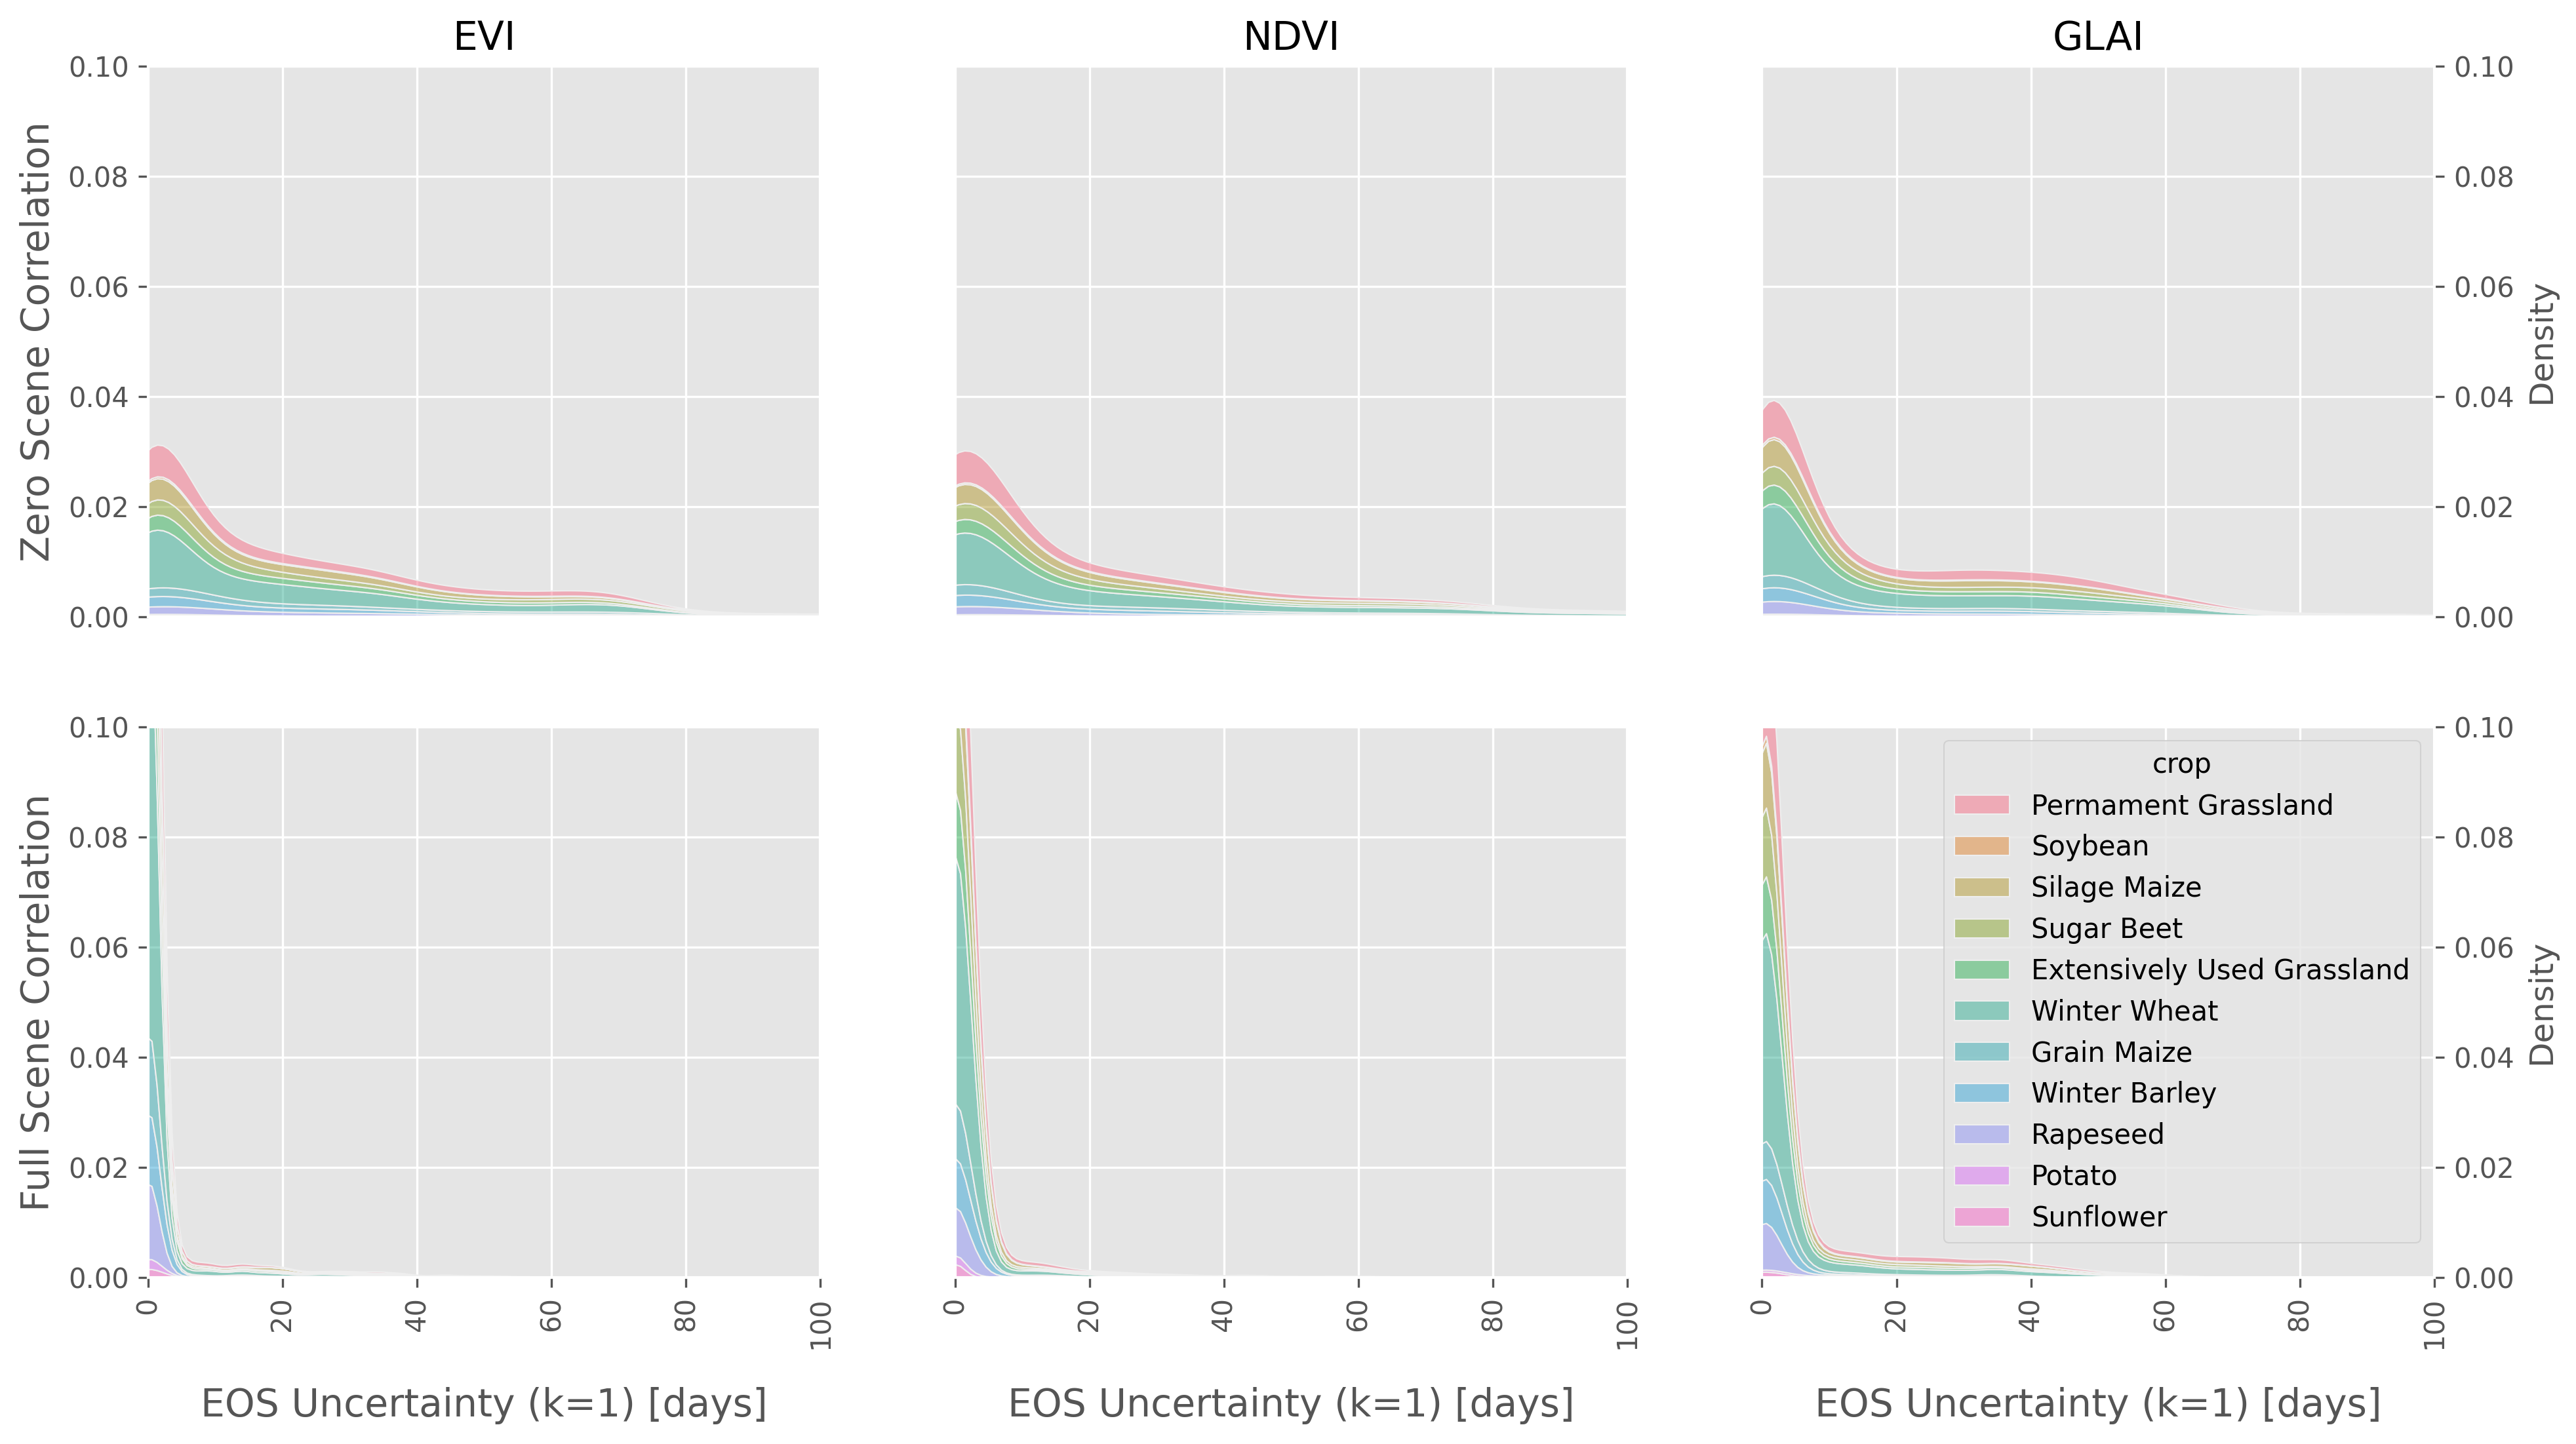
\includegraphics[width=1.0\textwidth]{eos_times_uncertainty.png}
    \caption{Kernel-based relative uncertainty distributions in End of Season (EOS) for \gls{EVI} (left column), \gls{NDVI} (middle column), and \gls{GLAI} (right column) color-coded by crop-type. The top row shows the results of the  \gls{MC} runs with zero inter-scene correlation; the bottom row the results assuming full inter-scene correlation.}
    \label{fig:eos-uncertainty}
\end{figure*}

\subsubsection{Length of Season}

Uncertainty in \gls{LOS} (Figure \ref{fig:los-uncertainty}) reflected shifts in \gls{SOS} and \gls{EOS} due to propagated uncertainties. Again, in the fully correlated case (Fig \ref{fig:los-uncertainty}, bottom row) uncertainties were low and hence the number of days the seasons gets longer or shorter was small, whereas the larger uncertainties in case of of zero inter-scene correlation caused larger shifts in \gls{LOS} (Fig \ref{fig:los-uncertainty}, top row).

In the uncorrelated case (Fig \ref{fig:los-uncertainty}, top row) all three time series sources showed a peak between one and 20 days with median uncertainties ranging from nine days (\gls{NDVI}  in potatoes) to 28 days (\gls{EVI}  and \gls{GLAI} in the grasslands). The right shoulder of the uncertainty distributions was broad and declined only smoothly towards zero. Thus, 95\% percent of the uncertainties were between 60 days (\gls{EVI}  in sunflower) and 78 days (\gls{EVI}  in permanent grassland and sugar beet). The secondary peak evident in \gls{SOS} and \gls{EOS} uncertainty distributions was pronounced in \gls{GLAI} but not in \gls{EVI} and NDVI.

LOS uncertainties were low in case of full inter-scene error correlation. The uncertainty distributions (Fig \ref{fig:los-uncertainty}, bottom row) showed a peak close to zero with a broader dispersion of values towards higher uncertainties in the case of GLAI. Median uncertainties were less than one day for all crops for the two spectral indices and one day in the case of GLAI. The values of the 95\% percentile ranged from 24 days (\gls{EVI}  in potatoes) to 59 days (\gls{NDVI}  in permanent grassland).

\begin{figure*}
    \centering
    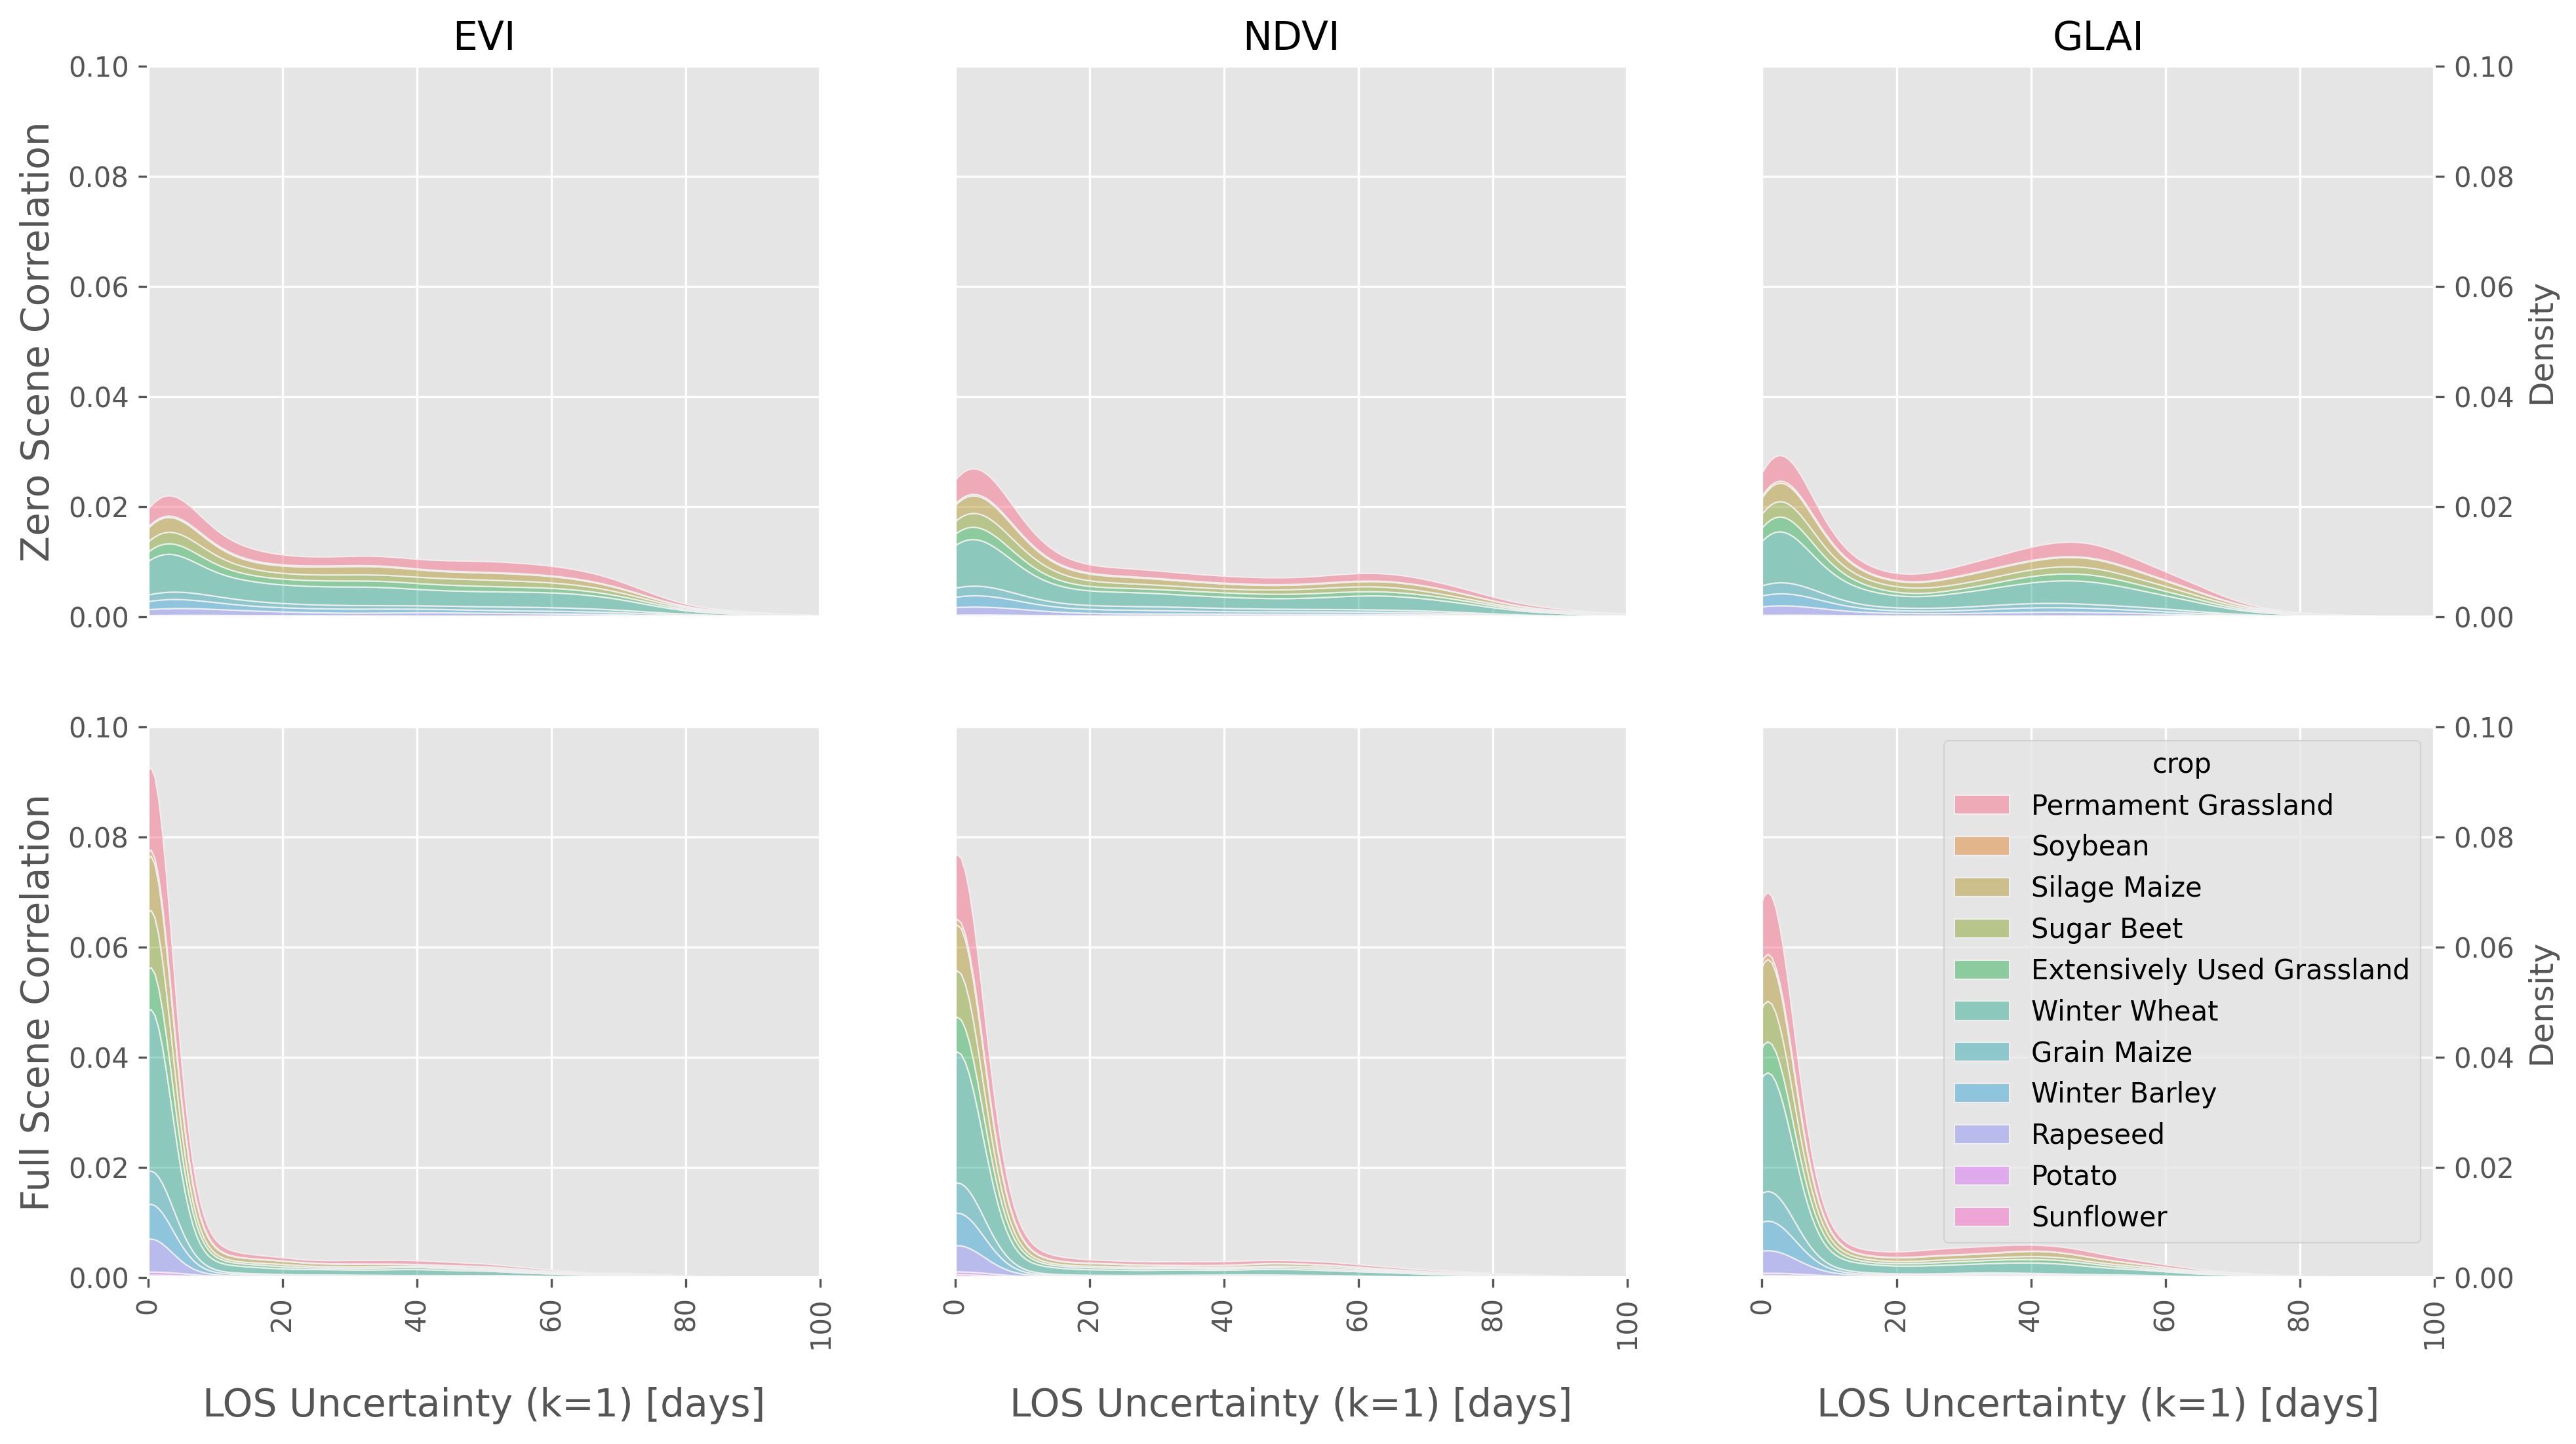
\includegraphics[width=1.0\textwidth]{length_of_season_uncertainty.png}
    \caption{Kernel-based relative uncertainty distributions in Length of Season (LOS) for \gls{EVI} (left column), \gls{NDVI} (middle column), and \gls{GLAI} (right column) color-coded by crop-type. The top row shows the results of the  \gls{MC} runs with zero inter-scene correlation; the bottom row the results assuming full inter-scene correlation.}
    \label{fig:los-uncertainty}
\end{figure*}

\section{Discussion}
\label{sec:unc_discussion}

\subsection{Interpretation of Results}
\subsubsection{Scene Classification Layer Uncertainty}

The \gls{SCL} product is robust to radiometric uncertainty. High uncertainties only occur at class boundaries (Figure \ref{fig:figure3-scl_uncertainty}). Namely the cloud shadow class showed the lowest confidence score, i.e., the highest class assignment uncertainties. We assume that the spectral indices and thresholds used were selected so that a broad number of different spectra are assigned to a class \citep{muller-wilm_sentinel-2_2013}. The class "Vegetation" (SCL class 4), for instance, includes contrasting vegetation types such as coniferous forests or crop canopies. The modification due to the radiometric uncertainty is smaller than the spectral within-class variability. Consequently, radiometric uncertainty has little influence. Only at the transition between classes, where spectral mixing effects are expected or vegetation is overlaid by translucent clouds does uncertainty cause changes in class assignments. Although the uncertainty analysis does not provide an indication of the accuracy of the \gls{SCL} product, the areas identified as uncertain in the \gls{S2} scenes are consistent with findings from validation studies: \cite{louis_sentinel-2_2019} attested only limited accuracy of Sen2Cor in more complex scenarios, especially for cloud shadow detection, and thus under conditions where uncertainty is also higher. \cite{liu_clouds_2019} compared different cloud detection algorithms in \gls{S2} data and found that the \gls{SCL} product gave inadequate results when it comes to cloud delineation. For example, translucent cloud edges were misclassified, which is consistent with the finding that pixels in these regions have high \gls{SCL} uncertainty. This suggests that applying a spatial buffer around cloud and shadow pixels might lower the occurrence of undetected atmospheric artifacts.

\subsubsection{Vegetation Indices and \gls{GLAI} Uncertainty}

EVI and \gls{NDVI} (Figures \ref{fig:ww-rel-unc-box} and \ref{fig:ww-timeseries-and-uncertainty}) have clearly lower relative uncertainty and show smaller spatio-temporal variability compared to GLAI.

In \gls{NDVI} we assume band rationing (Equation \ref{eq:ndvi}) to cancel out random errors, such as those from sensor noise, to a large degree. Still, normalization is accompanied by saturation at high biomass levels \citep{prabhakara_evaluating_2015}. Non-rationing indices like \gls{EVI} avoid saturation and have an increased sensitivity at high biomass values \citep{huete_overview_2002}. However, a basic assumption of the \gls{EVI} is that the satellite data are mostly noise-free. Due to inherent radiometric uncertainties in the blue, red, and infrared channels, this assumption is not fully met. Over vegetated areas, random sources of uncertainty dominate in the blue and red bands, where systematic effects play a smaller role due to the low radiance level. Systematic effects originate, for example, from straylight during sensor calibration. In the NIR band systematic and random effects occur nearly equal due to the higher radiance level of green vegetation. Therefore, \gls{EVI} is influenced by, both, systematic and random sources of uncertainty. Consequently, the higher relative uncertainties in \gls{EVI} compared to \gls{NDVI} can be explained. In NDVI, the saturation effect at high biomass values causes the uncertainty of the NIR band alone to dominate during this phase. For low biomass levels, the red band additionally contributes to the systematic uncertainty component. Thus, relative uncertainty in \gls{NDVI} reaches a minimum and maximum at the time of maximum and minimum green biomass accumulation, respectively. In \gls{EVI} all three bands contribute to the total uncertainty during the period of maximum greenness. The decrease of the absolute uncertainty in \gls{EVI} before and after the greenness maximum (Fig \ref{fig:ww-timeseries-and-uncertainty}, middle row left) can be explained by the removal of the canopy background targeted in the \gls{EVI} formula (Equation \ref{eq:evi}), which increasingly dominates the spectral properties as the plants mature. In mathematical terms the numerator becomes smaller and the denominator bigger. This limits the overall impact of uncertainties since the resulting \gls{EVI} values are small in any case when the canopy is not at its greenness peak.

GLAI is a physiological parameter derived from the inversion of a physically based radiative transfer model. It is therefore based on the entire spectral information and, hence, the uncertainties from all \gls{S2} bands. Furthermore, the inversion of the radiative transfer equation is ill-posed \citep{zurita-milla_visualizing_2015}. Using the median of the 100 simulated pixel spectra with the lowest spectral RMSE is an approach to solve the inverse problem. We assume to eliminate random sources of uncertainty to some extent. Still, the RMSE is a similarity measure that gives equal weight to all spectral bands. Thus, bands dominated by random uncertainty effects (low radiance levels) are weighted the same as bands where random and systematic effects occur to similar degrees (red edge and NIR bands). We hypothesize that the increase in reflectance in the red-edge and NIR bands as the growing season progresses conditions a greater weighting of the systematic uncertainties of these, synchronously increasing the absolute uncertainty in GLAI.

Differences found between the crops revealed that potato exhibited the highest median uncertainty values while the grasslands showed lowest median uncertainties. This can be explained by the number of observations that include plant and soil background, which in case of potatoes is high because the plants are grown in dams that are separated by trenches with usually little green canopy cover. Simply put, row crops such as potatoes violate the assumptions of the turbid medium PROSAIL model. As explained by the example of uncertainty dynamics in wheat (see above), the relative uncertainty is higher at higher biomass levels. This is also evident in the plot of spatio-temporal variability of uncertainty in potato (Figure \ref{fig:potato-timeseries-and-uncertainty}). Grassland (Figures \ref{fig:permanent-grassland-timeseries-and-uncertainty} and \ref{fig:ext-used-grassland-timeseries-and-uncertainty}) is always-green, so relative uncertainties are constantly low.

\subsubsection{LSP Uncertainty}
\label{subsec:discussion-lsp-uncertainty}

Inter-scene correlation determines \gls{LSP} uncertainty. If uncertainties are uncorrelated among \gls{S2} scenes, \gls{LSP} uncertainties are higher than if the they are fully correlated. In other words: If uncertainties are fully correlated, the \gls{LSP} retrieval approach based on seasonal amplitude thresholds is robust against propagated radiometric uncertainty and the impact on \gls{LSP} metrics is small.

Full inter-scene correlation ($\alpha = 1$) biases the time series. The series is shifted in either positive or negative y-axis direction by a constant factor (up- and downward arrows in Figure \ref{fig:figure2-workflow}b). Although the absolute amount of the shift scales for each data point differently because uncertainties in the spectral indices and \gls{GLAI} are not constant over time (see Section \ref{subsec:ndvi-evi-glai-uncertainty}), the shape of the curve is largely preserved. Furthermore, the impact on the \gls{LSP} metrics is dampened by using a relative threshold instead of absolute numbers. In contrast, when assuming zero error correlation ($\alpha = 0$) among the \gls{S2} scenes, each data point in the time series can be shifted in a different direction along the y-axis. In addition, the shift is not by a constant factor for the entire time series. Consequently, different values for the seasonal amplitude may be obtained and the timing of the \gls{LSP} metrics can differ between  \gls{MC} scenario runs.

A closer look at Figures \ref{fig:sos-uncertainty} to \ref{fig:los-uncertainty} shows differences between the crop types and between EVI, \gls{NDVI} and GLAI. Depending on the shape of the growth curve, even small changes can have larger effects on the \gls{LSP} calculation: Soybeans, for example, have a well-defined growth curve whose ascending and descending branches have a steep gradient. In contrast, the ascending branch of winter cereals is less well defined in the spectral indices, since the actual growth period starts in autumn of the previous year and the canopy appears green early in spring. Thus, if the growth curve is well accented, uncertainty has less influence because small changes in the time series values have less influence on \gls{LSP} estimation.

This points to a problem with the TIMESAT approach: The seasonal amplitude is meaningful if the green-up and brown-down branches are symmetric and a single clear maximum exists. However, the approach reaches its limit in the presence of strong asymmetries and thus can produce implausible results for \gls{SOS} and EOS. This could be an explanation for the secondary peak evident in the \gls{SOS} and \gls{EOS} uncertainty distributions (Figures \ref{fig:sos-uncertainty} and \ref{fig:eos-uncertainty}): If time series are asymmetric or have multiple peaks, uncertainty can cause shifts in \gls{SOS} and \gls{EOS} by several tens of days, which is reflected in the uncertainty distribution. Since the secondary peak occurs in all time series and all crops, we assume that incorrect labels (main crop reported by the farmer was wrong) of the parcels as well as spectral mixed pixel effects could have an influence.

\subsubsection{An Educated Guess about Inter-scene Error Correlation}

The question that follows from Section \ref{subsec:discussion-lsp-uncertainty} is which of the two inter-scene error correlation assumptions is closer to reality. While we cannot give a definitive answer at this point, considerations of the multi-temporal behavior of the uncertainty contributors in the \gls{S2-RUT} (see box in Figure \ref{fig:unc-diagram}, top left) allow a first guess based on \cite{gorrono_radiometric_2017, gorrono_providing_2018}.

For example, some sources of uncertainty are not correlated between scenes. These include the instrument noise, as well as the analog-to-digital quantization and the L1C image quantization into a 12bit floating point (radiance measurement) and 16bit integer system (stored reflectance factors), respectively. Furthermore, we assume that cross-talk and the stability of the dark-signal are uncorrelated between the scenes as residuals of signal correction.

This contrasts with effects that are correlated between scenes. It is known that the random part of the out-of-field (OOF) straylight has a pattern on the scan line of the \gls{MSI} detector array, which should be independent of the scene. Likewise, the systematic part of the OOF straylight is partially correlated between scenes, since the OOF only changes partially over time. For the diffuser absolute knowledge, there is a strong correlation over the entire time span since the pre-flight \gls{BRDF} model is common to all scenes. The interpolation of the \gls{BRDF} at different solar angles is considered not to significantly modify the error correlation between scenes. In contrast, for the diffuse cosine effect associated with micro-vibrations and thermal cycling, the inter-scene correlation is broken with recalibration, which occurs approximately every 18 days. The gamma correction, which includes corrections for non-linearity and non-uniformity, exhibits high correlation between scenes that are radiometrically similar because the uncertainty budget of this contributor depends on the radiance level. Consequently, the effect is less correlated for scenes that are radiometrically less similar. Therefore, the inter-scene correlation of gamma correction depends on the development of vegetation over time.

In summary, we assume that uncertainties between scenes tend to be correlated rather than uncorrelated. The actual uncertainties in the \gls{LSP} metrics might therefore be more likely in the range of values from the  \gls{MC} run of the zero inter-scene correlation. Still, the degree of inter-scene correlation is most likely a function of time. This means inter-scene correlation might not be constant over the growing season and be coupled with the phenological development of vegetation. Thus, our assumption needs to be further investigated.

\subsection{Significance of Radiometric Uncertainty in \gls{LSP} studies}

As shown in Section \ref{subsec:lsp-metrics}, the inter-scene error correlation has an impact on the uncertainty in the \gls{LSP} metrics. In case of full error correlation among the \gls{S2} scenes the uncertainties are mostly small. In case of uncorrelated errors, the uncertainties are clearly higher. Especially for fast growing crops like maize, uncertainties in \gls{SOS} of the order of $\ge10$ days imply large physiological differences between the determined \gls{SOS} dates. This is important when \gls{LSP} metrics are used to detect phenological shifts, for example to study the effects of climate change on plant growth \citep{garonna_variability_2016} or to quantify differences in the onset of phenological stages for wider areas \citep{nietupski_spatiotemporal_2021} or among varieties of the same crop. If the uncertainties are of a similar order of magnitude or even significantly larger than the expected phenological shifts, in the worst case no reliable statement can be made. For example, using MODIS time series for China for the period 2001 to 2014 as an example, \cite{luo_spatiotemporal_2017} were able to show that the variability in \gls{SOS} and \gls{EOS} expressed as a single standard deviation at the pixel level ranges from 0 to greater than 30 days. This is in the order of magnitude of the uncertainty for the case without error correlation (Figures \ref{fig:sos-uncertainty} and \ref{fig:eos-uncertainty} top row). Furthermore, the identified uncertainties in \gls{LOS} are not negligible, especially when \gls{LOS} is used as a proxy for vegetation productivity. For instance, \cite{park_changes_2016} reported an increase in \gls{LOS} of 2.6 days per decade for continental-scale \gls{LSP} retrieval in Northern America from Global Inventory Modeling
and Mapping Studies (GIMMS) NDVI. This increase in \gls{LOS} is slightly larger than the uncertainties in the fully correlated case (see Figure \ref{fig:los-uncertainty} bottom row) but clearly smaller than uncertainty estimates from the uncorrelated scenario runs (Figure \ref{fig:los-uncertainty} top row).

In addition, comparing radiometric uncertainty to other sources of uncertainties in \gls{LSP} retrieval that have already been investigated is important. For example, \cite{younes_all_2021} and \cite{van_bussel_effects_2011} found that changes in spatial aggregation can cause differences in \gls{LSP} metrics greater than 60 days, using mangrove forests and agricultural cropland, respectively. This exceeds the uncertainties identified from radiometry. In this regard \cite{helman_land_2018} highlights the effect of spectral mixing due to coarse spatial resolution: Changes in species composition could cause a similar change in the spectral properties of a pixel as an actual change in \gls{LSP} \citep{chen_mixed_2018}. Another source of uncertainty is introduced by the choice of the time series model: \cite{lara_assessing_2016} were able to show, using crop and grassland phenology from MODIS data, that uncertainties in \gls{SOS} and \gls{LOS} can range from 20 to 50 days based on the choice and parameterization of the time series model.

\subsection{Limitations}
\label{subsec:limitations}

As Figure \ref{fig:unc-diagram} shows, radiometry is one out of many sources of uncertainty that make up the total uncertainty budget of \gls{LSP} metrics. Since radiometric uncertainty affects all steps of \gls{EO} processing chains, such as AC or scene classification, quantifying and propagating radiometric uncertainties is an important first step. However, this also means that in further steps, sources of uncertainty have to be quantified, which are currently ignored ($\mu(0)$ in Figure \ref{fig:unc-diagram}). 

In terms of computational requirements, the proposed  \gls{MC} framework is rather slow and resource intensive. Preferably, uncertainties would be propagated analytically using the chain rule of uncertainty propagation. However, this requires knowledge about error covariance matrices and sensitivity coefficients. Currently, this information is hardly available in the \gls{EO} domain thus hampering the advancement of \gls{EO} as a measurement science as claimed by \cite{mittaz_applying_2019}.

Furthermore, the link to agronomically relevant estimates of phenological development in crops such as the BBCH scale - a decimal scale for crop development comparable to the scale developed by \cite{zadoks_decimal_1974} - is currently not given. Therefore, future research should focus on the impact of radiometric uncertainty on more advanced phenological metrics such as the start of heading in wheat \citep{harfenmeister_detecting_2021}. With the present work we provide a baseline to address these points thoroughly. Therefore, we published the calculated uncertainties in the L2B products (\gls{EVI} , NDVI, GLAI) as a data set for this study.

\section{Conclusions}
\label{sec:unc_conclusions}

We proposed a framework for propagating radiometric uncertainties in \gls{S2} L1C \gls{TOA}reflectance factors along an \gls{EO} data processing chain into \gls{LSP} metrics. The framework follows GUM specifications and demonstrates how uncertainties output from the \gls{S2-RUT} can be propagated into higher level \gls{EO} products. Not only did we trace radiometric uncertainties but also showed how radiometric uncertainty is embedded in the overall uncertainty budget of \gls{LSP} metrics.

Our results for various agricultural crops reveal that \gls{NDVI} and \gls{EVI} are more robust to radiometric uncertainty than \gls{GLAI} from RTM inversion. Still, this is not yet a statement on the suitability of spectral indices or physically-based crop traits for phenology assessment. This applies to all crops suggesting that no crop-specific uncertainty exists. The \gls{S2} \gls{SCL} product was mostly invariant to radiometric uncertainty, except for spectrally mixed pixels. These occur, for example, at cloud shadow edges or with translucent clouds. Furthermore, our results show that propagated radiometric uncertainty influences the timing of \gls{LSP} metrics in the order of a few days. In extreme cases, uncertainties can take up to a few weeks. Uncertainties in \gls{LSP} metrics should be taken into account when interpreting \gls{LSP} data or when comparing remotely sensed phenology estimates to ground observations. However, more in-depth research on inter-scene error correlation is needed to further assess the magnitude of uncertainty in \gls{LSP} metrics. In addition, sources of uncertainty not addressed in this study - e.g., from the AC - should be quantified.

Last, we would like to emphasize that the methods and findings of our research are fully reproducible as code and L2B data products are freely available. Thus, future research can follow up our approaches and elaborate on open questions - also with regard to other disciplines and geographical regions.

\section*{Code Availability}
Code used for the data processing and analysis is available at: \url{https://doi.org/10.5281/zenodo.6669854}.

\section*{Data Availability}
We provide standard uncertainties for NDVI, \gls{EVI} and \gls{GLAI} (L2B products) for an entire growing season as an output of the radiometric uncertainty propagation chain. The data is available at: \url{https://doi.org/10.3929/ethz-b-000574818}.

